\documentclass[
  man,
  longtable,
  nolmodern,
  notxfonts,
  notimes,
  colorlinks=true,linkcolor=blue,citecolor=blue,urlcolor=blue]{apa7}

\usepackage{amsmath}
\usepackage{amssymb}




\RequirePackage{longtable}
\RequirePackage{threeparttablex}

\makeatletter
\renewcommand{\paragraph}{\@startsection{paragraph}{4}{\parindent}%
	{0\baselineskip \@plus 0.2ex \@minus 0.2ex}%
	{-.5em}%
	{\normalfont\normalsize\bfseries\typesectitle}}

\renewcommand{\subparagraph}[1]{\@startsection{subparagraph}{5}{0.5em}%
	{0\baselineskip \@plus 0.2ex \@minus 0.2ex}%
	{-\z@\relax}%
	{\normalfont\normalsize\bfseries\itshape\hspace{\parindent}{#1}\textit{\addperi}}{\relax}}
\makeatother




\usepackage{longtable, booktabs, multirow, multicol, colortbl, hhline, caption, array, float, xpatch}
\usepackage{subcaption}


\renewcommand\thesubfigure{\Alph{subfigure}}
\setcounter{topnumber}{2}
\setcounter{bottomnumber}{2}
\setcounter{totalnumber}{4}
\renewcommand{\topfraction}{0.85}
\renewcommand{\bottomfraction}{0.85}
\renewcommand{\textfraction}{0.15}
\renewcommand{\floatpagefraction}{0.7}

\usepackage{tcolorbox}
\tcbuselibrary{listings,theorems, breakable, skins}
\usepackage{fontawesome5}

\definecolor{quarto-callout-color}{HTML}{909090}
\definecolor{quarto-callout-note-color}{HTML}{0758E5}
\definecolor{quarto-callout-important-color}{HTML}{CC1914}
\definecolor{quarto-callout-warning-color}{HTML}{EB9113}
\definecolor{quarto-callout-tip-color}{HTML}{00A047}
\definecolor{quarto-callout-caution-color}{HTML}{FC5300}
\definecolor{quarto-callout-color-frame}{HTML}{ACACAC}
\definecolor{quarto-callout-note-color-frame}{HTML}{4582EC}
\definecolor{quarto-callout-important-color-frame}{HTML}{D9534F}
\definecolor{quarto-callout-warning-color-frame}{HTML}{F0AD4E}
\definecolor{quarto-callout-tip-color-frame}{HTML}{02B875}
\definecolor{quarto-callout-caution-color-frame}{HTML}{FD7E14}

%\newlength\Oldarrayrulewidth
%\newlength\Oldtabcolsep


\usepackage{hyperref}




\providecommand{\tightlist}{%
  \setlength{\itemsep}{0pt}\setlength{\parskip}{0pt}}
\usepackage{longtable,booktabs,array}
\usepackage{calc} % for calculating minipage widths
% Correct order of tables after \paragraph or \subparagraph
\usepackage{etoolbox}
\makeatletter
\patchcmd\longtable{\par}{\if@noskipsec\mbox{}\fi\par}{}{}
\makeatother
% Allow footnotes in longtable head/foot
\IfFileExists{footnotehyper.sty}{\usepackage{footnotehyper}}{\usepackage{footnote}}
\makesavenoteenv{longtable}

\usepackage{graphicx}
\makeatletter
\newsavebox\pandoc@box
\newcommand*\pandocbounded[1]{% scales image to fit in text height/width
  \sbox\pandoc@box{#1}%
  \Gscale@div\@tempa{\textheight}{\dimexpr\ht\pandoc@box+\dp\pandoc@box\relax}%
  \Gscale@div\@tempb{\linewidth}{\wd\pandoc@box}%
  \ifdim\@tempb\p@<\@tempa\p@\let\@tempa\@tempb\fi% select the smaller of both
  \ifdim\@tempa\p@<\p@\scalebox{\@tempa}{\usebox\pandoc@box}%
  \else\usebox{\pandoc@box}%
  \fi%
}
% Set default figure placement to htbp
\def\fps@figure{htbp}
\makeatother


% definitions for citeproc citations
\NewDocumentCommand\citeproctext{}{}
\NewDocumentCommand\citeproc{mm}{%
  \begingroup\def\citeproctext{#2}\cite{#1}\endgroup}
\makeatletter
 % allow citations to break across lines
 \let\@cite@ofmt\@firstofone
 % avoid brackets around text for \cite:
 \def\@biblabel#1{}
 \def\@cite#1#2{{#1\if@tempswa , #2\fi}}
\makeatother
\newlength{\cslhangindent}
\setlength{\cslhangindent}{1.5em}
\newlength{\csllabelwidth}
\setlength{\csllabelwidth}{3em}
\newenvironment{CSLReferences}[2] % #1 hanging-indent, #2 entry-spacing
 {\begin{list}{}{%
  \setlength{\itemindent}{0pt}
  \setlength{\leftmargin}{0pt}
  \setlength{\parsep}{0pt}
  % turn on hanging indent if param 1 is 1
  \ifodd #1
   \setlength{\leftmargin}{\cslhangindent}
   \setlength{\itemindent}{-1\cslhangindent}
  \fi
  % set entry spacing
  \setlength{\itemsep}{#2\baselineskip}}}
 {\end{list}}
\usepackage{calc}
\newcommand{\CSLBlock}[1]{\hfill\break\parbox[t]{\linewidth}{\strut\ignorespaces#1\strut}}
\newcommand{\CSLLeftMargin}[1]{\parbox[t]{\csllabelwidth}{\strut#1\strut}}
\newcommand{\CSLRightInline}[1]{\parbox[t]{\linewidth - \csllabelwidth}{\strut#1\strut}}
\newcommand{\CSLIndent}[1]{\hspace{\cslhangindent}#1}





\usepackage{newtx}

\defaultfontfeatures{Scale=MatchLowercase}
\defaultfontfeatures[\rmfamily]{Ligatures=TeX,Scale=1}





\title{An Efficient Rotation-Sign-Permutation Algorithm to Solve
Rotational Indeterminacy in Bayesian Exploratory Factor Analysis}


\shorttitle{Efficient RSP Algorithm}


\usepackage{etoolbox}









\authorsnames[{1},{2}]{Ricardo Rey-Sáez,Javier Revuelta}







\authorsaffiliations{
{Department of Basic Psychology, Universidad Autónoma de
Madrid},{Department of Social Psychology and Methodology, Universidad
Autónoma de Madrid}}




\leftheader{Rey-Sáez and Revuelta}



\abstract{Posterior samples of factor loadings in Bayesian exploratory
factor analysis are not directly comparable across MCMC iterations due
to rotational indeterminacy. As a result, their posterior means are
typically close to zero because they cancel across rotationally
equivalent orientations, yielding uninterpretable factor loading
estimates. Alignment-based post-processing is therefore required, but
existing approaches face a trade-off: exact alignment methods do not
scale well beyond low-dimensional settings, whereas scalable
alternatives rely on approximations that can reduce accuracy. We
introduce an efficient version of the Rotation-Sign-Permutation (RSP)
algorithm of Papastamoulis and Ntzoufras (2022) that overcomes these
limitations by making exact alignment scalable to a large number of
factors. Simulations and empirical examples demonstrate that this
algorithm achieves higher alignment accuracy in high-dimensional
settings with negligible computational overhead. An optimized C++
implementation is available in the open-source R package
\texttt{BayesEFA}. }

\keywords{Bayesian exploratory factor analysis, Bayesian factor
models, label switching, rotational indeterminacy, post-processing.}

\authornote{\par{\addORCIDlink{Ricardo
Rey-Sáez}{0000-0001-6739-2035}}\par{\addORCIDlink{Javier
Revuelta}{0000-0003-4705-6282}} 
\par{ }
\par{This study was not preregistered. All data, models, and scripts
required to reproduce the results of this work are publicly available at
\url{https://github.com/RicardoReySaez/ERSP} and
\url{https://osf.io/4nyd7/}. The efficient-RSP algorithm is publicly
available in \texttt{BayesEFA} package, which can be installed from
\url{https://github.com/RicardoReySaez/BayesEFA}.  The authors declare
that they have no conflict of interest. This work was supported by the
Spanish Ministry of Science and Innovation grants PID2023-150830NB-I00
(to RRS) and PID2021-124885NB-I00 (to JR).   Author roles were
classified using the Contributor Role Taxonomy (CRediT;
\url{https://credit.niso.org}) as follows:  Ricardo
Rey-Sáez:   conceptualization, data curation, formal
analysis, investigation, methodology, project
administration, software, validation, visualization, writing -- original
draft, writing -- review \& editing; Javier
Revuelta:   conceptualization, methodology, supervision, writing --
review \& editing}
\par{Correspondence concerning this article should be addressed
to Ricardo Rey-Sáez, Department of Basic Psychology, Universidad
Autónoma de Madrid, Ivan Pavlov Street, 6, Fuencarral-El
Pardo, Madrid 28049, Spain, Email: \href{mailto:ricardoreysaez95@gmail.com}{ricardoreysaez95@gmail.com}}
}

\makeatletter
\let\endoldlt\endlongtable
\def\endlongtable{
\hline
\endoldlt
}
\makeatother
\RequirePackage{longtable}
\DeclareDelayedFloatFlavor{longtable}{table}

\urlstyle{same}



\usepackage{booktabs}
\usepackage{longtable}
\usepackage{array}
\usepackage{multirow}
\usepackage{wrapfig}
\usepackage{float}
\usepackage{colortbl}
\usepackage{pdflscape}
\usepackage{tabu}
\usepackage{threeparttable}
\usepackage{threeparttablex}
\usepackage[normalem]{ulem}
\usepackage{makecell}
\usepackage{xcolor}
\let\openbox\relax
\usepackage[ruled,vlined,linesnumbered]{algorithm2e}
\makeatletter
\@ifpackageloaded{caption}{}{\usepackage{caption}}
\AtBeginDocument{%
\ifdefined\contentsname
  \renewcommand*\contentsname{Table of contents}
\else
  \newcommand\contentsname{Table of contents}
\fi
\ifdefined\listfigurename
  \renewcommand*\listfigurename{List of Figures}
\else
  \newcommand\listfigurename{List of Figures}
\fi
\ifdefined\listtablename
  \renewcommand*\listtablename{List of Tables}
\else
  \newcommand\listtablename{List of Tables}
\fi
\ifdefined\figurename
  \renewcommand*\figurename{Figure}
\else
  \newcommand\figurename{Figure}
\fi
\ifdefined\tablename
  \renewcommand*\tablename{Table}
\else
  \newcommand\tablename{Table}
\fi
}
\@ifpackageloaded{float}{}{\usepackage{float}}
\floatstyle{ruled}
\@ifundefined{c@chapter}{\newfloat{codelisting}{h}{lop}}{\newfloat{codelisting}{h}{lop}[chapter]}
\floatname{codelisting}{Listing}
\newcommand*\listoflistings{\listof{codelisting}{List of Listings}}
\usepackage{amsthm}
\theoremstyle{plain}
\newtheorem{theorem}{Theorem}[section]
\theoremstyle{plain}
\newtheorem{lemma}{Lemma}[section]
\theoremstyle{remark}
\AtBeginDocument{\renewcommand*{\proofname}{Proof}}
\newtheorem*{remark}{Remark}
\newtheorem*{solution}{Solution}
\newtheorem{refremark}{Remark}[section]
\newtheorem{refsolution}{Solution}[section]
\makeatother
\makeatletter
\makeatother
\makeatletter
\@ifpackageloaded{caption}{}{\usepackage{caption}}
\@ifpackageloaded{subcaption}{}{\usepackage{subcaption}}
\makeatother

% From https://tex.stackexchange.com/a/645996/211326
%%% apa7 doesn't want to add appendix section titles in the toc
%%% let's make it do it
\makeatletter
\xpatchcmd{\appendix}
  {\par}
  {\addcontentsline{toc}{section}{\@currentlabelname}\par}
  {}{}
\makeatother

%% Disable longtable counter
%% https://tex.stackexchange.com/a/248395/211326

\usepackage{etoolbox}

\makeatletter
\patchcmd{\LT@caption}
  {\bgroup}
  {\bgroup\global\LTpatch@captiontrue}
  {}{}
\patchcmd{\longtable}
  {\par}
  {\par\global\LTpatch@captionfalse}
  {}{}
\apptocmd{\endlongtable}
  {\ifLTpatch@caption\else\addtocounter{table}{-1}\fi}
  {}{}
\newif\ifLTpatch@caption
\makeatother

\begin{document}

\maketitle




\setlength\LTleft{0pt}




Factor models are a widely used latent-variable approach that represent
dependence among observed variables through a smaller set of unobserved
variables. They are foundational in modern psychometrics
(\citeproc{ref-vanBork2024}{Bork et al., 2024};
\citeproc{ref-joreskog1969general}{Jöreskog, 1969};
\citeproc{ref-thurstone1947multiple}{Thurstone, 1947}) and also serve as
a workhorse for covariance matrix estimation in high-dimensional
settings (\citeproc{ref-bhattacharya2011sparse}{Bhattacharya \& Dunson,
2011}; \citeproc{ref-Fan2008}{Fan et al., 2008};
\citeproc{ref-Stevenson2025group}{Stevenson et al., 2025}). The standard
factor model assumes that, for each observation \(i\), the
\(J\)-dimensional response vector \(\mathbf{y}_i\) is expressed as
\begin{equation}\phantomsection\label{eq-01}{
\mathbf{y}_i = \boldsymbol\nu + \mathbf\Lambda\cdot\boldsymbol\eta_{i} + \boldsymbol\varepsilon_{i},
}\end{equation} where \(\boldsymbol\nu\in\mathbb{R}^J\) is the vector of
intercepts of the \(J\) observed variables,
\(\mathbf\Lambda\in\mathbb{R}^{J\times M}\) is the factor-loading
matrix, \(\boldsymbol\eta_i\in\mathbb{R}^M\) is the vector of latent
factor scores for observation \(i\), and
\(\boldsymbol\varepsilon_i\in\mathbb{R}^J\) captures idiosyncratic
variation not explained by the common factors. It is assumed that
\(\boldsymbol\eta_i\) and \(\boldsymbol\varepsilon_i\) are independent
latent variables with distributions
\(\boldsymbol\eta_i\sim \mathcal{MVN}\left(\boldsymbol 0,\;\mathbf{I}_M\right)\)
and
\(\boldsymbol{\varepsilon}_i\sim\mathcal{MVN}\left(\boldsymbol 0,\;\mathbf\Psi\right)\),
where \(\mathbf\Psi\in\mathbb{R}^{J\times J}\) is a diagonal matrix of
unique variances. In this paper, we focus on the unrestricted factor
model---also known as Exploratory Factor Analysis (EFA)---in which all
elements of \(\mathbf\Lambda\) are freely estimated.

Given the assumption of local independence, and letting
\(\boldsymbol\theta = (\boldsymbol\nu, \mathbf\Lambda, \mathbf\Psi)\)
denote the collection of structural parameters, the conditional
distribution of \(\mathbf{y}_i\) is given by
\begin{equation}\phantomsection\label{eq-02}{
\mathbf{y}_i \mid \boldsymbol\eta_i, \boldsymbol\theta \sim \mathcal{MVN}\!\left(\boldsymbol\nu + \mathbf\Lambda \cdot\boldsymbol\eta_i,\;\mathbf\Psi\right), 
}\end{equation} and integrating out \(\boldsymbol\eta_i\) yields the
corresponding marginal model,
\begin{equation}\phantomsection\label{eq-03}{
\mathbf{y}_i \mid \boldsymbol\theta \sim \mathcal{MVN}\!\left(\boldsymbol\nu,\;\mathbf\Sigma\right),
\qquad
\mathbf\Sigma = \mathbf\Lambda\cdot\mathbf\Lambda^\top + \mathbf\Psi.
}\end{equation}

Here, \(\boldsymbol\nu\) and \(\mathbf\Sigma\) are commonly referred to
as the model-implied mean vector and the model-implied covariance
matrix, respectively. Since \(\mathbf\Psi\) is diagonal, the covariance
structure among the observed variables---represented by the off-diagonal
elements of \(\mathbf\Sigma\)---is entirely governed by the term
\(\mathbf\Lambda\cdot\mathbf\Lambda^\top\).

The marginal representation of Equation~\ref{eq-03} is convenient
because it makes explicit what the data likelihood ``sees'': once the
latent factors are integrated out, the likelihood depends on
\(\mathbf{\Lambda}\) solely through the implied covariance
\(\mathbf{\Sigma}\). Consequently, any alternative loading matrix
\(\mathbf\Lambda^\bullet\) satisfying
\(\mathbf\Lambda^\bullet\cdot\mathbf\Lambda^{\bullet\top}=\mathbf\Lambda\cdot\mathbf\Lambda^\top\)
implies the same \(\mathbf\Sigma\) and yields an identical likelihood,
meaning \(\mathbf\Lambda\) is not uniquely identified\footnote{Although
  our focus is on the rotational non-identifiability of
  \(\mathbf\Lambda\), the uniqueness matrix \(\mathbf\Psi\) must also be
  identified. Throughout the paper, we assume \(M \leq (J-1)/2\) and
  that \(\mathbf\Lambda\) has no zero rows (i.e., each observed variable
  loads on at least one factor). These conditions are sufficient for
  \(\mathbf\Psi\) to be identifiable.}
(\citeproc{ref-anderson1956statistical}{Anderson \& Rubin, 1956};
\citeproc{ref-millsap2001statistical}{Millsap, 2001}).

This lack of uniqueness stems from the model's invariance under
orthogonal transformations. Specifically, for any orthogonal matrix
\(\mathbf{Q}\in\mathbb{R}^{M\times M}\) with
\(\mathbf{Q}\cdot\mathbf{Q}^\top=\mathbf{I}_M\), the rotated loadings
\(\mathbf\Lambda^\bullet = \mathbf\Lambda\cdot\mathbf{Q}\) automatically
satisfy \[
\mathbf\Lambda^\bullet\cdot (\mathbf\Lambda^\bullet)^\top = \mathbf\Lambda\cdot \mathbf{Q}\cdot(\mathbf\Lambda\cdot \mathbf{Q})^\top=\mathbf\Lambda\cdot \mathbf{Q}\cdot\mathbf{Q}^\top\cdot \mathbf\Lambda^\top = \mathbf\Lambda\cdot \mathbf{I}_M\cdot \mathbf\Lambda^\top= \mathbf\Lambda \cdot \mathbf\Lambda^\top,
\] and therefore leave \(\mathbf\Sigma\) unchanged. Note also that
simple column sign flips and permutations in \(\mathbf\Lambda\) are
themselves orthogonal transformations.

To resolve this ambiguity in frequentist factor analysis, rotational
indeterminacy is typically handled by choosing a rotation matrix
\(\mathbf{Q}\) designed to maximize interpretability. Common choices
include orthogonal rotations such as Varimax
(\citeproc{ref-kaiser1958varimax}{Kaiser, 1958}), which preserve
uncorrelated factors, and oblique rotations such as Oblimin
(\citeproc{ref-JennrichSampson1966}{Jennrich \& Sampson, 1966}), which
allow correlated factors. From the rotated solution, the final column
order and signs are typically fixed by simple conventions based on the
strongest loadings in \(\mathbf\Lambda^\bullet\), enabling researchers
to assign conceptual labels and directions that align with theoretical
expectations.

While this procedure yields a unique solution in the frequentist
framework, dealing with rotational indeterminacy is more intricate in
Bayesian factor analysis because the ambiguity persists at every
posterior draw (see
\citeproc{ref-papastamoulis2022identifiability}{Papastamoulis \&
Ntzoufras, 2022} for a comprehensive review). Since the likelihood is
invariant to orthogonal transformations, the posterior inherits this
symmetry and becomes multimodal, with multiple equivalent modes
corresponding to different orthogonal rotations. As an MCMC sampler
explores this posterior, it may move between equivalent modes, so the
rotation, column ordering, and sign configuration can vary arbitrarily
from one iteration to the next. In practice, averaging across draws
mixes incompatible modes, producing posterior means and intervals for
\(\mathbf\Lambda\) that are not substantively interpretable.

To address this challenge, the Bayesian literature has largely converged
on two broad approaches\footnote{A useful brief overview of available
  methods can be found in Papastamoulis and Ntzoufras
  (\citeproc{ref-papastamoulis2022identifiability}{2022}),
  Frühwirth-Schnatter et al.
  (\citeproc{ref-Fruxfchwirth-Schnatter2025}{2025}) and Poworoznek et
  al. (\citeproc{ref-Poworoznek2025}{2025})}. The first aims to impose
identifiability during sampling, for example through parameter
constraints (\citeproc{ref-aguilar2000bayesian}{Aguilar \& West, 2000};
\citeproc{ref-anderson1956statistical}{Anderson \& Rubin, 1956};
\citeproc{ref-geweke1996measuring}{Geweke \& Zhou, 1996}), or
specialized samplers that encourage a sparse and interpretable loading
structure (\citeproc{ref-Chen2021}{Chen, 2021};
\citeproc{ref-conti2014bayesian}{Conti et al., 2014};
\citeproc{ref-econometrics11040026}{Frühwirth-Schnatter et al., 2023},
\citeproc{ref-Fruxfchwirth-Schnatter2025}{2025}). The second, in
contrast, leaves the model unconstrained during sampling and resolves
rotational indeterminacy by post-processing the MCMC output, using
alignment algorithms that map posterior draws onto a common reference
orientation (\citeproc{ref-Asman2016}{Aßmann et al., 2016};
\citeproc{ref-erosheva2017dealing}{Erosheva \& Curtis, 2017};
\citeproc{ref-Fontanella2019}{Fontanella et al., 2019};
\citeproc{ref-Kaufmann2017}{Kaufmann \& Schumacher, 2017};
\citeproc{ref-Marin2005}{Marin et al., 2005};
\citeproc{ref-papastamoulis2022identifiability}{Papastamoulis \&
Ntzoufras, 2022}; \citeproc{ref-Poworoznek2025}{Poworoznek et al.,
2025}). The present work contributes to this second line by introducing
a new algorithm for the globally optimal joint alignment of posterior
draws. The method performs well in both low- and high-dimensional
settings and remains accurate and computationally tractable even with
many latent factors (e.g., \(M\geq 50\)), where an exact, globally
optimal alignment solution has previously been computationally out of
reach. The algorithm is implemented in C++ and is available in the R
package \texttt{BayesEFA} (\citeproc{ref-BayesEFA}{Rey-Sáez, 2026}).

In the remainder of this paper, we first review the main Bayesian
approaches proposed to address rotational indeterminacy in factor
models. We then introduce our alignment algorithm and summarize its
theoretical and computational properties. Next, we present two
simulation studies. The first compares our method with the exact
procedure of Papastamoulis and Ntzoufras
(\citeproc{ref-papastamoulis2022identifiability}{2022}) in
low-dimensional settings where exact solutions remain tractable, showing
that both approaches yield the same aligned solutions. The second
compares our method, as dimensionality increases, against MatchAlign
(\citeproc{ref-Poworoznek2025}{Poworoznek et al., 2025}), an approximate
approach reported to offer a favorable accuracy--efficiency trade-off.
In this setting, our method achieves higher alignment accuracy, while
differences in runtime are negligible. Finally, we illustrate the method
with two empirical applications.

\subsection{Bayesian Attempts to Resolve Rotational
Indeterminacy}\label{bayesian-attempts-to-resolve-rotational-indeterminacy}

\subsubsection{Identification through model
specification}\label{identification-through-model-specification}

A standard way to address rotational indeterminacy is to introduce model
constraints that prevent the MCMC sampler from visiting equivalent
rotated solutions. Anderson and Rubin
(\citeproc{ref-anderson1956statistical}{1956}) addressed this by
proposing a lower-triangular structure for \(\mathbf{\Lambda}\), where
elements above the main diagonal are fixed to zero. To resolve sign and
scale indeterminacy, this specification is typically completed by fixing
the diagonal elements to unity
(\citeproc{ref-aguilar2000bayesian}{Aguilar \& West, 2000};
\citeproc{ref-anderson1956statistical}{Anderson \& Rubin, 1956}) or
constraining them to be positive
(\citeproc{ref-geweke1996measuring}{Geweke \& Zhou, 1996}), yielding
what is often referred to as a positive lower-triangular (PLT)
parameterization. While PLT has been widely used in Bayesian latent
variable modeling (\citeproc{ref-fokoue2003mixtures}{Fokoué \&
Titterington, 2003}; \citeproc{ref-Gronau2020}{Gronau et al., 2020};
\citeproc{ref-lopes2004bayesian}{Lopes \& West, 2004};
\citeproc{ref-lucas2006sparse}{Lucas et al., 2006};
\citeproc{ref-revuelta2022bayesian}{Revuelta et al., 2022};
\citeproc{ref-Revuelta2017}{Revuelta \& Ximénez, 2017}), it imposes a
strict dependency on variable order. Since the first observed variables
effectively anchor the factor space, the resulting inference becomes
sensitive to the ordering of the input data
(\citeproc{ref-bhattacharya2011sparse}{Bhattacharya \& Dunson, 2011};
\citeproc{ref-lopes2004bayesian}{Lopes \& West, 2004}), an issue that
becomes especially consequential when these anchor variables are weak
indicators of the underlying factors
(\citeproc{ref-Carvalho2008}{Carvalho et al., 2008}). Moreover, such
constraints can introduce additional multimodality and hinder mixing,
complicating MCMC convergence diagnostics
(\citeproc{ref-erosheva2017dealing}{Erosheva \& Curtis, 2017}), while
small changes in the zero pattern can lead to non-comparable solutions
and convergence issues (\citeproc{ref-millsap2001statistical}{Millsap,
2001}).

To move beyond PLT identification, a broad family of model-based
alternatives tries to identify \(\mathbf\Lambda\) in a less restrictive
way, allowing structure to emerge during estimation. Examples include
latent indicator formulations that select which variables load on which
factors (\citeproc{ref-conti2014bayesian}{Conti et al., 2014};
\citeproc{ref-Mavridis2014}{Mavridis \& Ntzoufras, 2014}), one-step
Bayesian regularized EFA approaches (\citeproc{ref-Chen2021}{Chen,
2021}), embedded rotation steps (\citeproc{ref-rockova2016fast}{Ročková
\& George, 2016}), scale-invariant spike-and-slab priors on standardized
loadings (\citeproc{ref-Quintero2024}{Quintero et al., 2024}), unordered
generalized lower-triangular parameterizations
(\citeproc{ref-econometrics11040026}{Frühwirth-Schnatter et al., 2023},
\citeproc{ref-Fruxfchwirth-Schnatter2025}{2025}), rotation-invariant
parameterizations that fix a canonical orientation
(\citeproc{ref-nirwan19a}{Nirwan \& Bertschinger, 2019}) or infinite
factor models, which allow an effectively unbounded number of latent
factors by using increasing shrinkage priors that progressively shrink
redundant columns of \(\mathbf\Lambda\) toward zero
(\citeproc{ref-bhattacharya2011sparse}{Bhattacharya \& Dunson, 2011};
\citeproc{ref-Knowles2011}{Knowles \& Ghahramani, 2011};
\citeproc{ref-Legramanti2020}{Legramanti et al., 2020};
\citeproc{ref-rockova2016fast}{Ročková \& George, 2016}). Although these
strategies are designed to identify \(\mathbf\Lambda\), posterior draws
are still not directly comparable. Column permutations and sign switches
can occur across iterations, so post-processing is necessary before
\(\mathbf\Lambda\) can be meaningfully summarized. This contrasts
sharply with posterior alignment, where identification is resolved
entirely after sampling.

\subsubsection{Identification through posterior
alignment}\label{identification-through-posterior-alignment}

Identification through posterior alignment resolves rotational
indeterminacy as a post-processing step, letting the MCMC sampler
explore the full set of equivalent rotated solutions. Rather than
modifying the model, the priors, or the sampling scheme, posterior
alignment changes only how posterior output is summarized: it reorders
and reorients the draws of \(\mathbf\Lambda\) by matching columns and
fixing signs so that draws become directly comparable. Because no
identifying constraints are imposed on \(\mathbf\Lambda\) during
sampling, the PLT-related identification issues discussed in the
previous subsection become largely irrelevant. As a result, posterior
alignment provides a conceptually simple framework that is
straightforward to implement in empirical settings.

Although several post-processing algorithms have been proposed for this
task (see \citeproc{ref-Poworoznek2025}{Poworoznek et al., 2025}, for a
brief review), here we focus on Procrustes-based approaches, which
formalize alignment by mapping each draw onto a common reference
configuration (\citeproc{ref-Schonemann1966Procrustes}{Schönemann,
1966}). Let \(\mathbf\Lambda^{(t)}\in\mathbb{R^{J\times M}}\) denote the
loading matrix at posterior draw \(t=1,\dots,T\). Posterior alignment
aims to find, for each draw, an orthogonal transformation that maps
\(\mathbf\Lambda^{(t)}\) into a common latent reference space. The
orthogonal Procrustes problem provides a natural formalization of this
goal: given a reference loading matrix
\(\mathbf\Lambda^\star\in\mathbb{R}^{J\times M}\), we seek, for each
\(t\), an orthogonal matrix
\(\mathbf{Q}^{(t)}\in\mathbb{R}^{M\times M}\) that minimizes the
Frobenius discrepancy between \(\mathbf{\Lambda}^{(t)}\cdot\mathbf{Q}\)
and \(\mathbf\Lambda^{\star}\),
\begin{equation}\phantomsection\label{eq-04}{
\mathbf{Q}^{(t)} = \arg\min_{\mathbf{Q}\in\mathcal{Q}_M}\left\|\mathbf{\Lambda}^{(t)}\cdot\mathbf{Q} - \mathbf{\Lambda}^\star\right\|^2_F,
}\end{equation} where \(\mathcal{Q}_M\) denotes the set of all
\(M \times M\) orthogonal matrices and \(\|\cdot\|_F\) is the Frobenius
norm.

The Procrustes objective in Equation~\ref{eq-04} underlies the Weighted
Orthogonal Procrustes (WOP) method proposed by Aßmann et al.
(\citeproc{ref-Asman2016}{2016}). While the formulation above assumes a
fixed reference matrix \(\mathbf\Lambda^\star\), WOP treats the
reference as part of the solution: starting from an initial
\(\mathbf\Lambda^\star\) estimated from the unconstrained MCMC output,
it alternates between (1) computing, for each draw, the orthogonal
transformation \(\mathbf{Q}^{(t)}\) that minimizes the Procrustes loss
relative to the current \(\mathbf\Lambda^\star\) and (2) updating
\(\mathbf\Lambda^\star\) using the estimator implied by the newly
aligned draws, until convergence to a fixed point. Subsequent work,
however, has noted that WOP can overestimate the number of factors in
overfitted models
(\citeproc{ref-papastamoulis2022identifiability}{Papastamoulis \&
Ntzoufras, 2022}) and may become numerically unstable in
high-dimensional settings (\citeproc{ref-Poworoznek2025}{Poworoznek et
al., 2025}).

To address alignment more efficiently, Papastamoulis and Ntzoufras
(\citeproc{ref-papastamoulis2022identifiability}{2022}) propose a
two-step strategy that separates the continuous rotational ambiguity
from the discrete label ambiguity. In the first stage, each posterior
draw is rotated to simple structure via Varimax, yielding
Varimax-rotated loadings \(\tilde{\mathbf\Lambda}^{(t)}\) that select a
canonical orientation within the equivalence class of orthogonally
rotated solutions. Once this continuous degree of freedom is fixed, the
remaining indeterminacy is purely discrete: the columns of
\(\tilde{\mathbf\Lambda}^{(t)}\) can still be permuted, and each column
can still flip sign. Accordingly, the goal becomes to find a
signed-permutation alignment matrix \(\mathbf{A}^{(t)}\) such that
\begin{equation}\phantomsection\label{eq-05}{
\mathbf{A}^{(t)} = \arg\min_{\mathbf{A}\in\mathcal{A}_M}\left\|\mathbf{\tilde\Lambda}^{(t)}\cdot\mathbf{A} - \mathbf{\Lambda}^\star\right\|^2_F,
}\end{equation} where \(\mathcal{A}_M\) denotes the set of all
\(M\times M\) signed permutation matrices. Any
\(\mathbf{A}\in\mathcal{A}_M\) can be decomposed as
\(\mathbf{A}=\mathbf{P}\cdot\mathbf{S}\), where
\(\mathbf{P}\in\mathcal{P}_M\) is a permutation matrix and
\(\mathbf{S}\in\mathcal{S}_M\) is a diagonal sign matrix with
\(s_m\in\{-1,1\}\). The reference \(\mathbf{\Lambda}^\star\) is obtained
using the same iterative logic as in WOP, alternating between (1)
alignment under the current \(\mathbf{\Lambda}^\star\) and (2) an update
of \(\mathbf{\Lambda}^\star\) based on the newly aligned draws.

A key advantage of this discretization is that Equation~\ref{eq-05}
admits an exact global optimum over the space of signed permutations. In
Papastamoulis and Ntzoufras
(\citeproc{ref-papastamoulis2022identifiability}{2022}), this optimum is
obtained by enumerating the \(2^M\) sign configurations and, for each
one, solving the optimal column matching as an assignment problem
(implemented via branch and bound method,
\citeproc{ref-Little1963}{Little et al., 1963}). They refer to this
procedure as the exact Rotation-Sign-Permutation (RSP) method, whose
main limitation is its computational cost. Since this method requires
solving \(2^M\) assignment problems, exact alignment is only practical
for small \(M\) (roughly \(M\leq 10\)); beyond that, the exponential
scaling makes the procedure quickly prohibitive
(\citeproc{ref-papastamoulis2022identifiability}{Papastamoulis \&
Ntzoufras, 2022}; \citeproc{ref-Poworoznek2025}{Poworoznek et al.,
2025}).

This computational challenge motivates approximate post-processing
schemes. Papastamoulis and Ntzoufras
(\citeproc{ref-papastamoulis2022identifiability}{2022}) propose two
simulated-annealing variants (``RSP-full-SA'' and ``RSP-partial-SA'')
that offer a practical approximate alternative in high-dimensional
settings. More recently, Poworoznek et al.
(\citeproc{ref-Poworoznek2025}{2025}) introduced MatchAlign, which
retains the same two-stage decomposition: Varimax first to fix the
continuous rotational degree of freedom, followed by a discrete step for
sign and label switching. The key difference is that MatchAlign uses a
fixed reference \(\mathbf{\Lambda}^\star\) rather than updating it
iteratively. The reference is selected directly from the Varimax-rotated
draws as a representative configuration, chosen as the draw
\(\mathbf{\tilde\Lambda}^{(t)}\) with median condition number
\(\kappa\left(\tilde{\mathbf\Lambda}\right)=\sigma_{\max}\left(\tilde{\mathbf\Lambda}\right) / \sigma_{\min}\left(\tilde{\mathbf\Lambda}\right)\),
where \(\sigma_{\max}\) and \(\sigma_{\min}\) denote the largest and
smallest singular values of \(\tilde{\mathbf\Lambda}\). Each draw is
then aligned to \(\mathbf{\Lambda}^\star\) via a greedy column-by-column
matching procedure. In simulations, Poworoznek et al.~report that
MatchAlign is consistently more accurate than ``RSP-full-SA'' and often
approaches exact RSP. In their empirical illustration, it performs best
at \(M=25\); at \(M=50\), it continues to yield stable aligned draws,
whereas ``RSP-full-SA'' does not successfully align the draws and WOP
becomes numerically unstable and fails to converge.

In short, existing approaches force a compromise between exactness,
scalability, and numerical stability. What is still missing is a method
that delivers an exact solution in the RSP sense while remaining
feasible for large \(M\), avoids the numerical fragility sometimes
reported for WOP, and does not incur the computational cost of exact or
annealed RSP, all while preserving the practical speed of MatchAlign. In
the next section, we introduce an algorithm designed to meet these
requirements.

\subsection{Efficient Rotation-Sign-Permutation
Algorithm}\label{efficient-rotation-sign-permutation-algorithm}

We now present the theoretical basis of our approach. The key idea is
that we can determine the sign flips after solving the column matching,
because the objective function in Equation~\ref{eq-05} can be defined to
automatically reflect the optimal sign of each candidate pair of columns
in \(\mathbf{\tilde\Lambda}\) and \(\mathbf{\Lambda}^\star\).
Lemma~\ref{lem-signs} shows that the sign-optimized distance depends
only on the absolute inner product between columns. This reduces the
discrete alignment step to a standard Linear Assignment Problem (LAP),
as formalized in Theorem~\ref{thm-main}, which yields the optimal column
permutation. The specific signs are then recovered deterministically
from the (non-absolute) inner products for the matched pairs.

\begin{lemma}[Optimal Sign for a Matched Column
Pair]\protect\hypertarget{lem-signs}{}\label{lem-signs}

Let \(\tilde{\lambda} \in \mathbb{R}^J\) and
\(\lambda^\star \in \mathbb{R}^J\) be two arbitrary vectors. We seek a
sign \(s \in \{-1, 1\}\) that minimizes the squared Euclidean distance
\(\|s\cdot\tilde{\lambda} - \lambda^\star\|_2^2\). Then, an optimal sign
is given by \begin{equation}\phantomsection\label{eq-06}{
s^\star\in\arg\min_{s\in\{-1,1\}}\left\|s\cdot\tilde\lambda - \lambda^\star\right\|^2_2 =
\begin{cases}
\operatorname{sign}\!\left(\langle \tilde{\lambda},\lambda^\star\rangle\right), & \text{if }\langle \tilde{\lambda},\lambda^\star\rangle\neq 0,\\[3pt]
\{-1,1\}, & \text{if }\langle \tilde{\lambda},\lambda^\star\rangle = 0,
\end{cases}
}\end{equation} where \(\langle \cdot,\cdot\rangle\) denotes the
Euclidean inner product. Moreover, the minimized value admits the closed
form \begin{equation}\phantomsection\label{eq-07}{
\min_{s\in\{-1,1\}}\left\|s\cdot\tilde\lambda - \lambda^\star\right\|^2_2 = \big\|\tilde\lambda\big\|^2_2 + \big\|\lambda^\star\big\|^2_2 - 2\cdot\left|\langle\tilde\lambda,\lambda^\star\rangle\right|
}\end{equation}

\end{lemma}

\begin{proof}
Expanding the squared norm yields:
\begin{equation}\phantomsection\label{eq-08}{
\big\|s\cdot\tilde{\lambda} - \lambda^\star\big\|_2^2 = \big\|s\cdot\tilde{\lambda}\big\|_2^2 + \big\|\lambda^\star\big\|_2^2 - 2\cdot \langle s\cdot\tilde{\lambda}, \lambda^\star \rangle = \big\|\tilde{\lambda}\big\|_2^2 + \big\|\lambda^\star\big\|_2^2 - 2\cdot s\cdot \langle \tilde{\lambda}, \lambda^\star \rangle,
}\end{equation} since
\(\big\|s\cdot\tilde{\lambda}\big\|_2^2=\big\|\tilde{\lambda}\big\|_2^2\).
The only term depending on \(s\) is
\(-2\cdot s\cdot\langle \tilde{\lambda},\lambda^\star\rangle\), which is
minimized by choosing \(s\) with the same sign as
\(\langle \tilde{\lambda},\lambda^\star\rangle\) when the latter is
nonzero. If \(\langle \tilde{\lambda},\lambda^\star\rangle=0\), both
\(s=-1\) and \(s=1\) yield the same value. Substituting the optimal
choice gives the minimum value
\begin{equation}\phantomsection\label{eq-09}{
\big\|\tilde{\lambda}\big\|_2^2+\big\|\lambda^\star\big\|_2^2 - 2\cdot\left|\langle \tilde{\lambda},\lambda^\star\rangle\right|.
}\end{equation}
\end{proof}

Using Lemma~\ref{lem-signs}, we rewrite the objective in terms of
sign-optimized column distances, so the joint minimization over
\((\mathbf{P}, \mathbf{S})\) reduces to a Linear Assignment Problem over
\(\mathbf{P}\).

\begin{theorem}[Exact Reduction of Signed-Permutation Alignment to a
Linear Assignment
Problem]\protect\hypertarget{thm-main}{}\label{thm-main}

Consider the problem of minimizing
\(\left\|\tilde{\mathbf\Lambda}\cdot\mathbf{P}\cdot\mathbf{S}-\mathbf{\Lambda}^\star\right\|_F^2\)
over permutation matrices \(\mathbf{P}\in\mathcal{P}_M\) and sign
matrices \(\mathbf{S}\in\mathcal{S}_M\). Let \(\tilde{\lambda}_k\) and
\(\lambda^\star_m\) denote the \(k\)-th and \(m\)-th columns of
\(\tilde{\mathbf\Lambda}\) and \(\mathbf\Lambda^\star\), respectively.
The global minimum is obtained by constructing the cost matrix
\(\mathbf{C} \in \mathbb{R}^{M \times M}\) with entries corresponding to
the sign-optimized distance between each pair of columns:
\begin{equation}\phantomsection\label{eq-10}{
C_{km}=\big\|\tilde\lambda_k\big\|_2^2 + \big\|\lambda^\star_m\big\|_2^2 - 2 \cdot \big|\langle\tilde\lambda_k,\lambda_m^\star\rangle\big|,
}\end{equation} and finding the permutation \(\nu^\star\) that minimizes
the total assignment cost: \begin{equation}\phantomsection\label{eq-11}{
\nu^\star = \arg\min_{\nu \in \mathcal{T}_M} \sum_{m=1}^M C_{\nu_m, m}.
}\end{equation}

Finally, the optimal signs are recovered by applying
Lemma~\ref{lem-signs} to each matched pair
\((\tilde{\lambda}_{\nu^\star_m}, \lambda^\star_m)\).

\end{theorem}

\begin{proof}
Let \(\nu \in \mathcal{T}_M\) be the permutation vector corresponding to
the permutation matrix \(\mathbf{P} \in \mathcal{P}_M\).
Right-multiplication by \(\mathbf{P}\) reorders columns, so the \(m\)-th
column of \(\tilde{\mathbf{\Lambda}}\cdot\mathbf{P}\) is
\(\tilde{\lambda}_{\nu_m}\) and
\begin{equation}\phantomsection\label{eq-12}{
\tilde{\mathbf{\Lambda}}\cdot\mathbf{P}=\big[\tilde{\lambda}_{\nu_1},\dots,\tilde{\lambda}_{\nu_M}\big].
}\end{equation}

Moreover, since \(\mathbf{S}=\operatorname{diag}(s_1,\dots,s_M)\) with
\(s_m\in\{-1,1\}\), right-multiplication by \(\mathbf{S}\) flips the
sign of each column independently:
\begin{equation}\phantomsection\label{eq-13}{
\tilde{\mathbf{\Lambda}}\cdot\mathbf{P}\cdot\mathbf{S}
=
\big[s_1\cdot\tilde{\lambda}_{\nu_1},\dots,s_M\cdot\tilde{\lambda}_{\nu_M}\big].
}\end{equation}

Writing
\(\mathbf{\Lambda}^\star=[\lambda^\star_1,\dots,\lambda^\star_M]\) and
using the identity \(\|\mathbf{X}\|_F^2=\sum_{m=1}^M\|x_m\|_2^2\) for a
matrix \(\mathbf{X}=[x_1,\dots,x_M]\), we obtain the column-wise
decomposition \begin{equation}\phantomsection\label{eq-14}{
\left\|\tilde{\mathbf\Lambda}\cdot\mathbf{P}\cdot\mathbf{S}-\mathbf{\Lambda}^\star\right\|_F^2
= \sum_{m=1}^M \left\| s_m\cdot\tilde{\lambda}_{\nu_m}-\lambda_m^\star \right\|_2^2.
}\end{equation}

For any fixed permutation \(\nu\), each term in the sum can be minimized
independently with respect to \(s_m \in \{-1, 1\}\). By
Lemma~\ref{lem-signs}, the minimum value of the \(m\)-th term is exactly
\(C_{\nu_m,m}\). Consequently, since the minimal distance is already
absorbed by \(C_{\nu_m,m}\) without needing to determine whether the
optimal sign is \(+1\) or \(-1\), the remaining minimization over
\(\mathbf{P}\) reduces to \begin{equation}\phantomsection\label{eq-15}{
\nu^\star \in \arg\min_{\nu \in \mathcal{T}_M} \sum_{m=1}^M C_{\nu_m,m},
}\end{equation} which is a Linear Assignment Problem. Although the
assignment costs embed the optimal signs, their explicit values remain
undetermined at this stage and are finally recovered by applying
Lemma~\ref{lem-signs} to each matched pair
\((\tilde{\lambda}_{\nu^\star_m}, \lambda^\star_m)\).
\end{proof}

Our procedure targets the same objective function as the exact RSP
method of Papastamoulis and Ntzoufras
(\citeproc{ref-papastamoulis2022identifiability}{2022}), but it
leverages the reduction in Theorem~\ref{thm-main} to shift the
computational workload. Instead of enumerating the \(2^M\) sign
configurations and solving a separate assignment problem for each one,
we embed the sign-optimized distances directly into the cost matrix and
solve a single LAP with the Hungarian algorithm
(\citeproc{ref-Kuhn1955Hungarian}{Kuhn, 1955}). Once the columns are
matched, the explicit signs are recovered deterministically, setting
\(s^\star_m=1\) to break ties when an inner product is exactly zero.
Algorithm \ref{alg:efficient-rsp} summarizes the full procedure, which
is implemented in C++ and is publicly available through the R package
\texttt{BayesEFA}.

\vspace{1em}
\begin{algorithm}[t]
\linespread{1}\selectfont
\caption{Efficient Varimax--RSP algorithm to resolve rotational indeterminacy in Bayesian exploratory factor analysis}
\label{alg:efficient-rsp}
\linespread{1.4}\selectfont
\small
\SetAlgoVlined
\LinesNotNumbered
\DontPrintSemicolon
\KwIn{MCMC sample of loadings $\{\mathbf\Lambda^{(t)}\}_{t=1}^T$ and initial reference $\mathbf\Lambda^\star$}
\KwOut{Aligned loadings $\{\hat{\mathbf\Lambda}^{(t)}\}_{t=1}^T$ and final reference $\mathbf\Lambda^\star$}

\vspace{0.2em}
\textbf{Step 1: Varimax rotation}\;
\For{$t \gets 1$ \KwTo $T$}{
  $\tilde{\mathbf\Lambda}^{(t)} \gets \mathrm{Varimax}\!\left(\mathbf\Lambda^{(t)}\right)$\;
}

\vspace{0.2em}
\textbf{Step 2: Signed-permutation alignment (exact over $\mathcal{A}_M$ via LAP)}\;

\Repeat{\textit{no improvement in the objective function}
$\left(\sum_{t=1}^T \sum_{m=1}^M C^{(t)}_{\nu^{(t)}_m,m}\right)$ \textit{is observed}}{

  \For{$t \gets 1$ \KwTo $T$}{

    \textbf{2.1. Cost matrix with optimal sign embedded}\;
    \For{$k \gets 1$ \KwTo $M$}{
      \For{$m \gets 1$ \KwTo $M$}{
        $C^{(t)}_{km}\gets\|\tilde{\lambda}^{(t)}_{k}\|_2^2+\|\lambda^\star_m\|_2^2-2\cdot\big|\langle \tilde{\lambda}^{(t)}_{k},\lambda^\star_m\rangle\big|$\;
      }
    }

    \textbf{2.2. Column matching via LAP}\;
    $\nu^{(t)}\gets \arg\min_{\nu\in\mathcal T_M}\sum_{m=1}^M C^{(t)}_{\nu_m,m}$\;
    Build $\mathbf P^{(t)}$ from $\nu^{(t)}$\;

    \textbf{2.3. Optimal signs for the chosen assignment}\;
    \For{$m \gets 1$ \KwTo $M$}{
      \eIf{$\langle \tilde{\lambda}^{(t)}_{\nu^{(t)}_m},\lambda^\star_m\rangle \neq 0$}{
        $s^{(t)}_m\gets \mathrm{sign}\!\left(\langle \tilde{\lambda}^{(t)}_{\nu^{(t)}_m},\lambda^\star_m\rangle\right)$\;
      }{
        $s^{(t)}_m \gets 1$\;
      }
    }
    $\mathbf S^{(t)}\gets\mathrm{diag}(s^{(t)}_1,\dots,s^{(t)}_M)$\;

    \textbf{2.4. Align posterior draw}\;
    $\hat{\mathbf\Lambda}^{(t)}\gets \tilde{\mathbf\Lambda}^{(t)}\cdot\mathbf P^{(t)}\cdot\mathbf S^{(t)}$\;
  }

  Update reference $\mathbf\Lambda^\star \gets \frac{1}{T}\sum_{t=1}^T \hat{\mathbf\Lambda}^{(t)}$\;
}

\end{algorithm}
\vspace{1em}

\subsection{Performance Evaluation}\label{performance-evaluation}

We evaluate the performance of our algorithm through two simulation
studies and two empirical illustrations. By Theorem~\ref{thm-main}, our
method targets the same global optimum as the exact RSP formulation of
Papastamoulis and Ntzoufras
(\citeproc{ref-papastamoulis2022identifiability}{2022}); accordingly,
Study 1 serves as an implementation check in low-dimensional settings
where exact RSP remains feasible, showing that both procedures yield the
same aligned solutions. Study 2 benchmarks our exact method against
MatchAlign (\citeproc{ref-Poworoznek2025}{Poworoznek et al., 2025}), a
strong and scalable baseline for high-dimensional alignment. We do not
include the simulated-annealing variants of RSP, as they are explicitly
intended as stochastic approximations to the objective that our method
already optimizes exactly, and are therefore less informative for the
present comparison. Across studies, we compare alignment accuracy,
numerical stability, and runtime, showing that our algorithm achieves
exact alignment while remaining scalable. Finally, the empirical
illustrations demonstrate that the method yields stable and
interpretable posterior summaries in applied research. The code required
to reproduce all simulations and empirical analyses is publicly
available at \url{https://osf.io/4nyd7/} and
\url{https://github.com/RicardoReySaez/ERSP}.

\section{Simulation Studies}\label{simulation-studies}

\subsection{Method}\label{method}

\subsubsection{Design}\label{design}

Following the simulation setup of Poworoznek et al.
(\citeproc{ref-Poworoznek2025}{2025}), we conducted two simulation
studies manipulating sample size (\(N\)), the number of latent factors
(\(M\)), the number of observed variables (\(J\)), and the
data-generating structure of the loading matrix (``Independent''
vs.~``Sparse''). In the ``Independent'' condition, we generated dense
loadings in which all observed variables loaded on all factors. In the
``Sparse'' condition, we generated a simple structure in which each item
had a single primary loading and no cross-loadings. In both scenarios,
non-zero loadings were drawn from a standard normal distribution, and
unique variances were drawn from an inverse-gamma distribution with
shape and scale parameters set to 1/2.

The first simulation study was designed to demonstrate the equivalence
between our efficient RSP algorithm and the exact RSP method from
Papastamoulis and Ntzoufras
(\citeproc{ref-papastamoulis2022identifiability}{2022}), tractable only
at low dimensionalities. For clarity, throughout the manuscript we refer
to the original method of Papastamoulis and Ntzoufras as RSP, and to our
efficient variant as E-RSP. To this end, we fixed the sample size at
\(N=500\) and varied the number of latent factors
\(M\in\{2,3,4,5,6,7\}\), the number of observed variables
\(J\in\{50,100\}\) and the data-generating scenario for the factor
loadings. This design yielded \(1 \times 6 \times 2 \times 2 = 24\)
conditions, with 20 replicated datasets generated under each condition.

The second simulation study was designed to compare the efficient RSP
algorithm with MatchAlign algorithm from Poworoznek et al.
(\citeproc{ref-Poworoznek2025}{2025}). We manipulated sample size
\(N \in \{100, 250, 500\}\), number of latent factors
\(M \in \{5, 10, 15, 20, 25, 30\}\), and total observed variables
\(J \in \{50, 100, 200\}\), under the same Independent and Sparse
loading scenarios. This full factorial design resulted in 3 × 6 × 3 × 2
= 108 conditions, with 100 replicated datasets generated under each
condition.

\subsubsection{Procedure}\label{procedure}

Both simulation studies were conducted in \texttt{R}
(\citeproc{ref-Rcite}{R Core Team, 2025}), version 4.5.0, using the
\texttt{SimDesign} package (\citeproc{ref-SimDesign}{Chalmers \& Adkins,
2020}) to ensure a fully reproducible simulation workflow. Observed
datasets were generated by sampling from a multivariate normal
distribution via the \texttt{rmvn} function from the \texttt{mvnfast}
package (\citeproc{ref-mvnfast}{Fasiolo, 2014}). For each replicate, we
followed the model and computational specifications of Poworoznek et al.
(\citeproc{ref-Poworoznek2025}{2025}): we fitted a Bayesian Gaussian
factor model with a Dirichlet-Laplace shrinkage prior using the
\texttt{linearDL} function from the \texttt{infinitefactor} package
(\citeproc{ref-infinitefactor}{Poworoznek, 2020}). We ran 11,000 MCMC
iterations, discarding the first 1,000 as burn-in and thinning every 10
iterations to obtain 1,000 posterior draws per condition. Finally, these
draws were aligned using our E-RSP algorithm, implemented in the
\texttt{R} package \texttt{BayesEFA}. In Study 1, we compared E-RSP
against the exact RSP algorithm implemented in \texttt{factor.switching}
(\citeproc{ref-papastamoulis2022identifiability}{Papastamoulis \&
Ntzoufras, 2022}), whereas in Study 2 we compared E-RSP against
MatchAlign as implemented in \texttt{infinitefactor}.

\subsubsection{Analysis}\label{analysis}

Across both simulation studies, we evaluated alignment performance using
a common set of metrics. In addition to runtime, we quantified alignment
accuracy with a rotation-invariant Frobenius discrepancy based on the
implied common covariance, as in Poworoznek et al.
(\citeproc{ref-Poworoznek2025}{2025}). Specifically, we compared (i) the
posterior mean of the implied common covariance,
\(\overline{\mathbf\Lambda\cdot\mathbf\Lambda^\top}\), with (ii) the
covariance implied by the posterior mean of the aligned loadings,
\(\overline{\mathbf\Lambda}_{\text{A}}\cdot\overline{\mathbf\Lambda}_{\text{A}}^\top\),
where \(\overline{\mathbf\Lambda}_{\text{A}}\) denotes the posterior
mean of the aligned draws: \begin{equation}\phantomsection\label{eq-16}{
\|\overline{\mathbf\Lambda\cdot\mathbf\Lambda^\top} - \overline{\mathbf\Lambda}_{\text{A}}\cdot\overline{\mathbf\Lambda}_{\text{A}}^\top\|_{F}
}\end{equation}

Since the model-explained covariance is identifiable and invariant to
orthogonal rotations, this discrepancy provides a direct measure of how
well alignment recovers a coherent posterior summary. To facilitate
comparison across conditions, we also report a relative error obtained
by normalizing Equation~\ref{eq-16} by
\(\overline{\mathbf\Lambda\cdot\mathbf\Lambda^\top}\),
\begin{equation}\phantomsection\label{eq-17}{
\frac{\|\overline{\mathbf\Lambda\cdot\mathbf\Lambda^\top} - \overline{\mathbf\Lambda}_{\text{A}}\cdot\overline{\mathbf\Lambda}_{\text{A}}^\top\|_{F}}{\|\overline{\mathbf\Lambda\cdot\mathbf\Lambda^\top}\|_F}. 
}\end{equation}

For Simulation Study 2, we included two additional indicators. First, we
compute Equation~\ref{eq-16} and Equation~\ref{eq-17} using the raw,
unaligned posterior draws to quantify baseline misalignment due to
rotational non-identifiability. By dividing this baseline by the error
of the aligned estimates, we derived an improvement ratio that
quantifies how many times the alignment increases precision relative to
the uncorrected output. Finally, we assess the mixing quality of the
post-processed chains using the Effective Sample Size (ESS). Both bulk
and tail ESS are reported, averaged across loading elements and
expressed as a percentage of the total number of posterior draws.

\subsection{Results}\label{results}

\subsubsection{Simulation Study 1}\label{simulation-study-1}

Consistent with Theorem~\ref{thm-main}, E-RSP matched RSP in every
condition: across replications, dimensionalities, and loading
structures, both methods produced identical aligned draws and therefore
identical absolute errors. Figure \ref{fig-rsp-agreement} confirms this
one-to-one agreement by plotting the absolute error estimates from E-RSP
against those from RSP, with all estimates falling on the identity line
(\(r=1.00\)). However, runtime differed sharply and diverged rapidly as
\(M\) increases. Table \ref{tab:simres_1} reports mean alignment time
(minutes) and speedup ratios, reflecting the expected combinatorial
scaling of RSP. For example, under the Sparse loading structure with
\(M=7\), RSP required about 28 minutes per replication, whereas E-RSP
completed the same alignment in under 0.01 minutes (about half a
second). This runtime gap in the highest-\(M\) condition translates into
speedup ratios ranging from 345 to more than 3,000, depending on the
loading structure and the number of observed variables.

\begin{figure}

\caption{\label{fig-rsp-agreement}Agreement of absolute fit errors
between Exact and Efficient RSP methods}

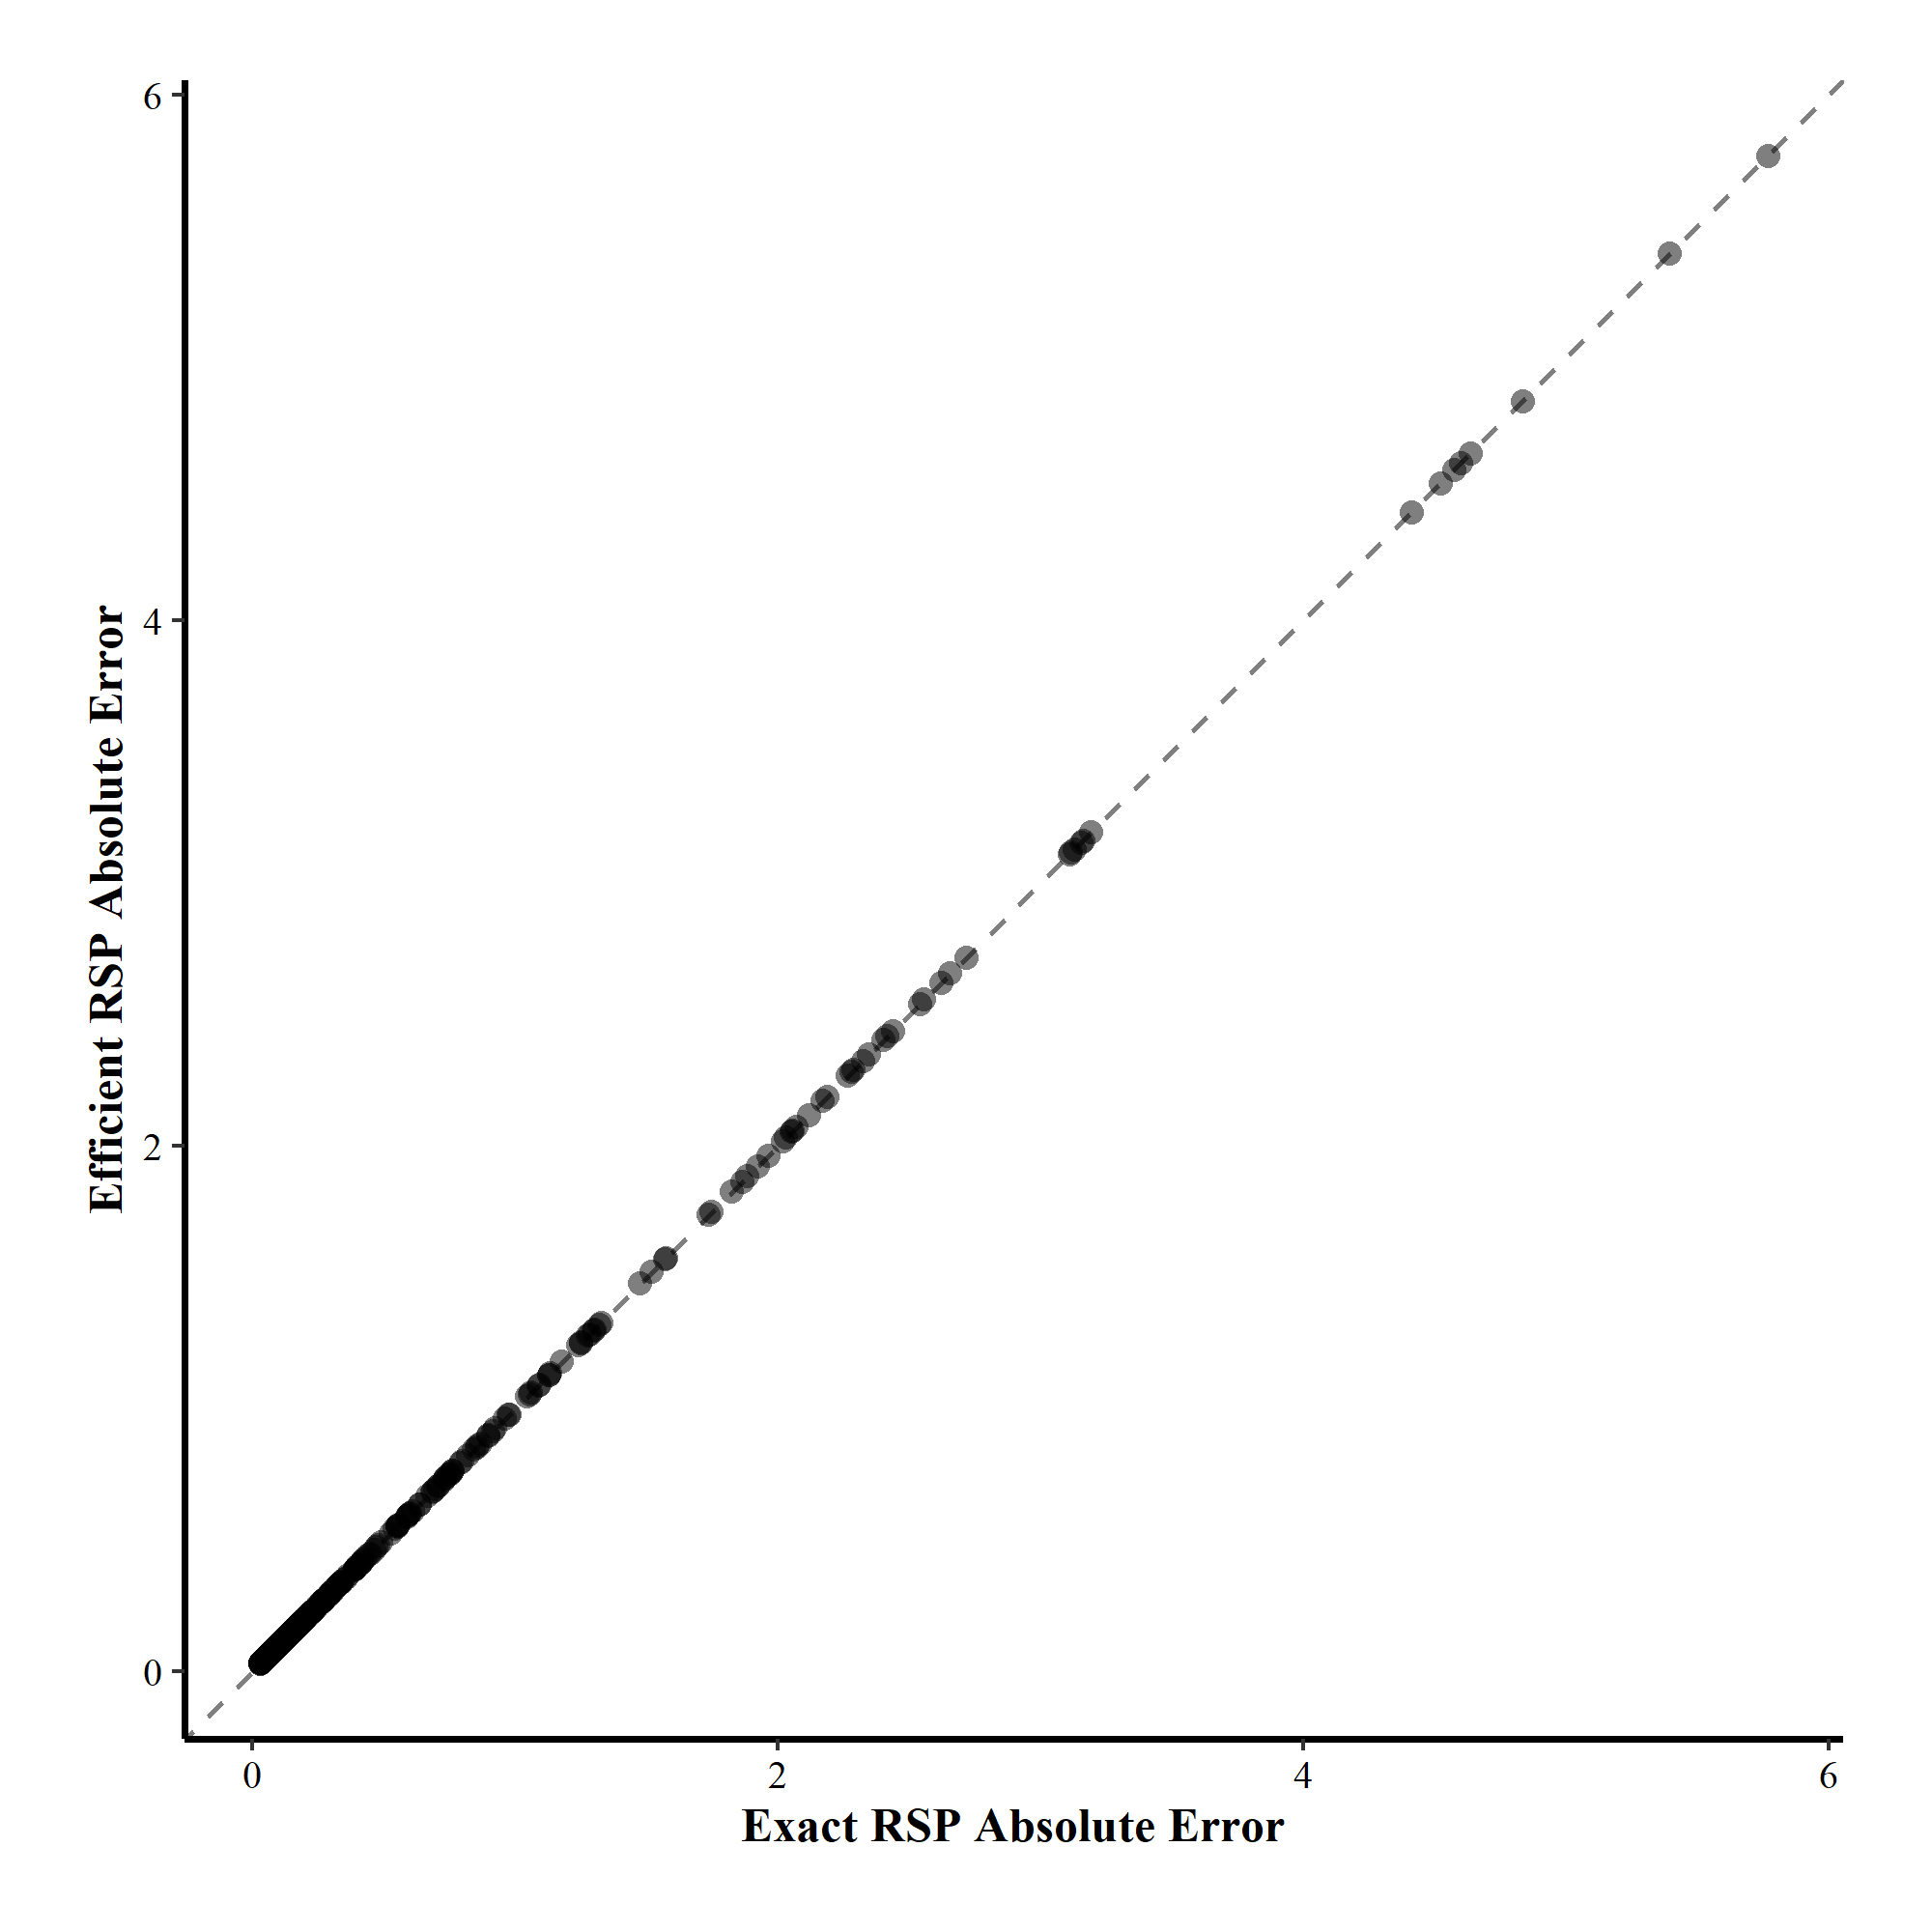
\includegraphics[width=5.3in,height=5.3in]{../Figures/RSP_agreement.png}

\end{figure}%

\begin{table}[!h]
\centering
\caption{\label{tab:simres_1}Computational performance comparison: Execution time (minutes) and speedup ratios comparing Exact and Efficient RSP methods.}
\centering
\begin{tabular}[t]{r@{\hspace{1.6cm}}>{\raggedleft\arraybackslash}p{1.6cm}>{\raggedleft\arraybackslash}p{1.6cm}>{\raggedleft\arraybackslash}p{1.6cm}c>{\raggedleft\arraybackslash}p{1.6cm}>{\raggedleft\arraybackslash}p{1.6cm}>{\raggedleft\arraybackslash}p{1.6cm}}
\toprule
\multicolumn{1}{c}{ } & \multicolumn{3}{c}{J = 50} & \multicolumn{1}{c}{ } & \multicolumn{3}{c}{J = 100} \\
\cmidrule(l{3pt}r{3pt}){2-4} \cmidrule(l{3pt}r{3pt}){6-8}
$M$ & RSP & E-RSP & Ratio &  & RSP & E-RSP & Ratio\\
\midrule
\addlinespace[0.5em]
\multicolumn{8}{l}{\textbf{Independent}}\\
\hspace{1em}2 & 0.483 & 0.010 & 49.081 &  & 0.539 & 0.016 & 34.565\\
\hspace{1em}3 & 1.301 & 0.021 & 62.247 &  & 1.038 & 0.027 & 38.804\\
\hspace{1em}4 & 2.859 & 0.028 & 103.043 &  & 2.334 & 0.040 & 58.811\\
\hspace{1em}5 & 5.915 & 0.030 & 200.347 &  & 6.871 & 0.055 & 124.849\\
\hspace{1em}6 & 11.828 & 0.039 & 300.577 &  & 10.752 & 0.068 & 158.804\\
\hspace{1em}7 & 24.774 & 0.046 & 533.741 &  & 29.762 & 0.086 & 345.231\\
\addlinespace[0.5em]
\multicolumn{8}{l}{\textbf{Sparse}}\\
\hspace{1em}2 & 0.467 & 0.004 & 115.222 &  & 0.423 & 0.005 & 83.492\\
\hspace{1em}3 & 0.962 & 0.005 & 203.257 &  & 0.944 & 0.007 & 137.441\\
\hspace{1em}4 & 2.008 & 0.005 & 406.395 &  & 1.972 & 0.007 & 265.525\\
\hspace{1em}5 & 4.170 & 0.006 & 720.984 &  & 4.202 & 0.008 & 497.265\\
\hspace{1em}6 & 9.420 & 0.007 & 1268.743 &  & 8.612 & 0.010 & 861.211\\
\hspace{1em}7 & 28.118 & 0.009 & 3141.687 &  & 18.511 & 0.012 & 1557.723\\
\bottomrule
\end{tabular}
\end{table}

These simulation results validate the LAP reformulation as a globally
optimal alternative to exhaustive search while reducing computational
cost by orders of magnitude. Across all conditions considered here,
E-RSP remains below 0.1 minutes, supporting its use in
higher-dimensional settings where exhaustive enumeration is infeasible.

\subsubsection{Simulation study 2}\label{simulation-study-2}

Table \ref{tab:simres_2_acc} summarizes accuracy results for MatchAlign
and E-RSP. Across all conditions, E-RSP achieves lower misfit than
MatchAlign on both absolute and relative accuracy metrics and yields
larger improvements over the unaligned baseline. This advantage persists
in the most demanding conditions. For instance, at the highest latent
dimensionality condition with \(M=30\), E-RSP reduces mean absolute
misfit from 30.88 (MatchAlign) to 23.66 and increases the relative fit
ratio from 2.07 to 2.70; under Independent loadings, the relative fit
ratio is 3.58 for E-RSP versus 2.96 for MatchAlign. As expected,
accuracy improves with larger \(N\) and deteriorates as \(M\) and \(J\)
increase, with Independent structures more challenging than Sparse ones.
In sum, E-RSP is more accurate than MatchAlign across the full
simulation design.

\renewcommand{\arraystretch}{0.9}

\begin{table}
\centering
\caption{\label{tab:simres_2_acc}Estimated marginal means of fit performance comparing MatchAlign (MA) and Efficient RSP (E-RSP) methods.}
\centering
\begin{threeparttable}
\begin{tabular}[t]{lcccccccccc}
\toprule
\multicolumn{1}{c}{ } & \multicolumn{3}{c}{Accuracy} & \multicolumn{1}{c}{ } & \multicolumn{3}{c}{Rel. Accuracy} & \multicolumn{1}{c}{ } & \multicolumn{2}{c}{Fit Ratio} \\
\cmidrule(l{3pt}r{3pt}){2-4} \cmidrule(l{3pt}r{3pt}){6-8} \cmidrule(l{3pt}r{3pt}){10-11}
Factor & Base & MA & E-RSP &  & Base & MA & E-RSP &  & MA & E-RSP\\
\midrule
\addlinespace[0.3em]
\multicolumn{11}{l}{\textbf{N}}\\
\hspace{1em}100 & 62.80 & 40.33 & \textbf{29.65} &  & 89.01 & 51.31 & \textbf{37.48} &  & 3.37 & \textbf{3.98}\\
\hspace{1em}250 & 21.86 & 10.13 & \textbf{7.83} &  & 76.13 & 28.11 & \textbf{21.65} &  & 6.96 & \textbf{7.54}\\
\hspace{1em}500 & 10.69 & 4.86 & \textbf{3.78} &  & 64.63 & 19.95 & \textbf{15.52} &  & 11.19 & \textbf{11.75}\\
\addlinespace[0.3em]
\multicolumn{11}{l}{\textbf{M}}\\
\hspace{1em}5 & 16.97 & 2.93 & \textbf{2.44} &  & 49.49 & 6.05 & \textbf{5.12} &  & 20.30 & \textbf{20.53}\\
\hspace{1em}10 & 27.64 & 9.33 & \textbf{6.99} &  & 70.80 & 18.15 & \textbf{13.96} &  & 9.55 & \textbf{10.20}\\
\hspace{1em}15 & 32.05 & 17.26 & \textbf{12.21} &  & 79.15 & 31.53 & \textbf{23.23} &  & 5.24 & \textbf{5.92}\\
\hspace{1em}20 & 35.24 & 22.89 & \textbf{16.71} &  & 83.80 & 41.28 & \textbf{30.62} &  & 3.40 & \textbf{4.06}\\
\hspace{1em}25 & 38.15 & 27.35 & \textbf{20.50} &  & 87.02 & 48.52 & \textbf{36.31} &  & 2.48 & \textbf{3.12}\\
\hspace{1em}30 & 40.66 & 30.88 & \textbf{23.66} &  & 89.27 & 53.21 & \textbf{40.05} &  & 2.07 & \textbf{2.70}\\
\addlinespace[0.3em]
\multicolumn{11}{l}{\textbf{J}}\\
\hspace{1em}50 & 9.85 & 4.16 & \textbf{3.01} &  & 85.38 & 33.24 & \textbf{24.47} &  & 6.39 & \textbf{7.21}\\
\hspace{1em}100 & 22.57 & 11.93 & \textbf{8.87} &  & 77.12 & 33.33 & \textbf{25.21} &  & 7.33 & \textbf{7.86}\\
\hspace{1em}200 & 62.93 & 39.24 & \textbf{29.39} &  & 67.27 & 32.80 & \textbf{24.97} &  & 7.81 & \textbf{8.20}\\
\addlinespace[0.3em]
\multicolumn{11}{l}{\textbf{Lambda}}\\
\hspace{1em}Independent & 33.42 & 22.58 & \textbf{17.03} &  & 62.67 & 34.99 & \textbf{25.89} &  & 2.96 & \textbf{3.58}\\
\hspace{1em}Sparse & 30.15 & 14.31 & \textbf{10.48} &  & 90.51 & 31.26 & \textbf{23.87} &  & 11.39 & \textbf{11.93}\\
\bottomrule
\end{tabular}
\begin{tablenotes}
\item \textit{Note.} 
\item Base denotes the baseline performance using unaligned draws. Accuracy is $\|\overline{\mathbf\Lambda\cdot\mathbf\Lambda^\top} - \overline{\mathbf\Lambda}_{\text{A}}\cdot\overline{\mathbf\Lambda}_{\text{A}}^\top\|_{F}$, and Rel. Accuracy is the same quantity divided by $\|\overline{\mathbf\Lambda\cdot\mathbf\Lambda^\top}\|_F$. Bold values indicate the best performing method for each condition (lowest values for Accuracy/Rel. Accuracy; highest values for Fit Ratio).
\end{tablenotes}
\end{threeparttable}
\end{table}

Table \ref{tab:simres_2_eff} reports sampling efficiency (bulk and tail
ESS, expressed as ESS/\(N_\text{draws}\)) and runtime for MatchAlign and
E-RSP. Across the full design, MatchAlign yields slightly higher ESS
values for both bulk and tail. However, E-RSP still achieves
consistently high ESS values that are unlikely to limit posterior
summaries in practice. These differences should be interpreted alongside
the accuracy results in Table \ref{tab:simres_2_acc}: higher ESS is not,
by itself, an advantage if it reflects more efficient sampling around a
less accurate post-processed solution. In this sense, MatchAlign tends
to mix marginally better, but around aligned summaries that are
systematically worse in fit than those obtained with E-RSP.

\begin{table}
\centering
\caption{\label{tab:simres_2_eff}Estimated marginal means for sampling efficiency (ESS) and computational time comparing MatchAlign (MA) and Efficient RSP (E-RSP).}
\centering
\begin{threeparttable}
\begin{tabular}[t]{lcccccccccc}
\toprule
\multicolumn{1}{c}{ } & \multicolumn{2}{c}{ESS Bulk} & \multicolumn{1}{c}{ } & \multicolumn{2}{c}{ESS Tail} & \multicolumn{1}{c}{ } & \multicolumn{4}{c}{Time (seconds)} \\
\cmidrule(l{3pt}r{3pt}){2-3} \cmidrule(l{3pt}r{3pt}){5-6} \cmidrule(l{3pt}r{3pt}){8-11}
Factor & MA & E-RSP &  & MA & E-RSP &  & MA & E-RSP & $\Delta$Time & Ratio\\
\midrule
\addlinespace[0.3em]
\multicolumn{11}{l}{\textbf{N}}\\
\hspace{1em}100 & \textbf{81.71} & 79.36 &  & \textbf{84.92} & 83.90 &  & \textbf{26.48} & 30.12 & 3.63 & 0.88\\
\hspace{1em}250 & \textbf{67.85} & 65.64 &  & \textbf{76.39} & 75.21 &  & \textbf{23.86} & 25.92 & 2.06 & 0.91\\
\hspace{1em}500 & \textbf{65.43} & 63.29 &  & \textbf{74.94} & 73.93 &  & \textbf{23.05} & 24.52 & 1.47 & 0.92\\
\addlinespace[0.3em]
\multicolumn{11}{l}{\textbf{M}}\\
\hspace{1em}5 & \textbf{66.60} & 66.28 &  & \textbf{75.91} & 75.82 &  & \textbf{2.72} & 2.74 & 0.02 & 0.99\\
\hspace{1em}10 & \textbf{67.14} & 65.93 &  & \textbf{75.68} & 75.12 &  & \textbf{7.71} & 8.00 & 0.29 & 0.94\\
\hspace{1em}15 & \textbf{70.29} & 68.22 &  & \textbf{77.80} & 76.72 &  & \textbf{16.95} & 18.03 & 1.09 & 0.91\\
\hspace{1em}20 & \textbf{73.14} & 70.30 &  & \textbf{79.72} & 78.28 &  & \textbf{27.12} & 29.55 & 2.43 & 0.88\\
\hspace{1em}25 & \textbf{75.51} & 72.15 &  & \textbf{81.23} & 79.61 &  & \textbf{39.94} & 44.35 & 4.41 & 0.87\\
\hspace{1em}30 & \textbf{77.27} & 73.70 &  & \textbf{82.17} & 80.54 &  & \textbf{52.36} & 58.45 & 6.10 & 0.86\\
\addlinespace[0.3em]
\multicolumn{11}{l}{\textbf{J}}\\
\hspace{1em}50 & \textbf{78.80} & 76.67 &  & \textbf{83.38} & 82.63 &  & \textbf{8.70} & 10.43 & 1.73 & 0.88\\
\hspace{1em}100 & \textbf{71.03} & 68.53 &  & \textbf{78.59} & 77.33 &  & \textbf{19.50} & 21.83 & 2.33 & 0.91\\
\hspace{1em}200 & \textbf{65.16} & 63.09 &  & \textbf{74.28} & 73.09 &  & \textbf{45.20} & 48.31 & 3.11 & 0.93\\
\addlinespace[0.3em]
\multicolumn{11}{l}{\textbf{Lambda}}\\
\hspace{1em}Independent & \textbf{54.27} & 50.56 &  & \textbf{68.87} & 66.93 &  & \textbf{37.16} & 39.54 & 2.38 & 0.95\\
\hspace{1em}Sparse & \textbf{89.05} & 88.30 &  & \textbf{88.63} & 88.43 &  & \textbf{11.77} & 14.17 & 2.39 & 0.87\\
\bottomrule
\end{tabular}
\begin{tablenotes}
\item \textit{Note.} 
\item ESS denotes Effective Sample Size. $\Delta$Time represents the average difference in time alignment between E-RSP and MA (calculated as Time E-RSP minus Time MA). The 'Ratio' column represents the relative speedup (Time MA / Time E-RSP). Bold values indicate the best performing method (highest for ESS; lowest for Time).
\end{tablenotes}
\end{threeparttable}
\end{table}

Runtimes are very close across methods, with a slight advantage for
MatchAlign, with time ratios ranging from 0.86 to 0.99 across all
conditions. This pattern is expected, as MatchAlign does not require an
iterative step to construct \(\mathbf\Lambda^\star\). However, the
absolute differences are small: even in the most demanding condition
(\(M=30\)), the mean runtime difference is only about six seconds per
replication. In practice, this few-second advantage is negligible given
the substantial gains in alignment accuracy provided by E-RSP.

In summary, the simulation results indicate that E-RSP is the preferred
alignment method over MatchAlign in this setting. E-RSP yields
systematically more accurate aligned solutions across the full design,
while maintaining adequate sampling efficiency for stable posterior
summaries. This accuracy gain comes at only a trivial computational
cost: on average, E-RSP requires 2.40 additional seconds per
replication, and even in the most demanding scenario the overhead is
only 6.10 seconds on average. Taken together, these results support
E-RSP as a practical choice for high-dimensional settings, effectively
enabling exact alignment without a meaningful runtime penalty.

\section{Empirical Illustrations}\label{empirical-illustrations}

\subsection{NHANES Data}\label{nhanes-data}

Our first empirical illustration reproduces the high-dimensional
chemical exposure analysis of Poworoznek et al.
(\citeproc{ref-Poworoznek2025}{2025}) using NHANES 2015--2016 data. For
a direct comparison, we follow their inclusion criteria and modeling
choices, publicly available at
\url{https://github.com/fedfer/Section_5_MatchAlign}. The dataset
contains \(J=107\) chemical exposure variables measured in \(N=4,468\)
individuals. As in Poworoznek et al., we fit a Bayesian factor model
under the Multiplicative Gamma Shrinkage Prior (MGSP,
\citeproc{ref-bhattacharya2011sparse}{Bhattacharya \& Dunson, 2011}),
which shrinks redundant factor dimensions toward zero in
high-dimensional settings. We consider the same two scenarios: \(M=25\)
factors (accounting for 65\% of total variance) and \(M=50\) factors
(reaching 85\% variance explained). The \(M=50\) specification is
particularly informative because it corresponds to the scenario where
existing post-processing methods have been reported to break down.

Table \ref{tab:NHANES_res} summarizes the NHANES re-analysis. At
\(M=25\), MatchAlign and E-RSP yield virtually identical posterior
summaries: both attain the same relative error (0.71\%) and similar ESS
values. The main difference is runtime. E-RSP completes alignment in
7.02 seconds, compared to 12.47 seconds for MatchAlign\footnote{Runtimes
  in the simulation study correspond to aligning \(\mathbf\Lambda\)
  only. In the NHANES re-analysis, we reproduce the pipeline in
  Poworoznek et al. (\citeproc{ref-Poworoznek2025}{2025}), where both
  the loading matrix \(\mathbf\Lambda\) and the latent scores
  \(\boldsymbol\eta\) are aligned. This is the default option in
  \texttt{infinitefactor} and modestly increases MatchAlign runtimes.},
without any loss in accuracy. At \(M=50\), E-RSP remains faster (19.15
vs.~29.25 seconds) and reduces the relative error from 1.68\% under
MatchAlign to 1.46\%. MatchAlign retains a modest ESS advantage, but
this occurs alongside a larger covariance reconstruction error. Overall,
E-RSP is the preferred option here, delivering equal or lower
reconstruction error with shorter runtime across both factor dimensions.

\begin{table}
\centering
\caption{\label{tab:NHANES_res}Performance metrics for the NHANES re-analysis}
\centering
\begin{threeparttable}
\begin{tabular}[t]{lccccccccc}
\toprule
\multicolumn{1}{c}{ } & \multicolumn{4}{c}{$M = 25$} & \multicolumn{1}{c}{ } & \multicolumn{4}{c}{$M = 50$} \\
\cmidrule(l{3pt}r{3pt}){2-5} \cmidrule(l{3pt}r{3pt}){7-10}
Method & Rel. Acc. & ESS$_B$ & ESS$_T$ & Time &  & Rel. Acc. & ESS$_B$ & ESS$_T$ & Time\\
\midrule
MA & 0.71 & 20.55 & 40.12 & 12.47 &  & 1.68 & 35.29 & 25.45 & 29.25\\
E-RSP & 0.71 & 20.41 & 39.93 & 7.02 &  & 1.46 & 33.26 & 20.70 & 19.15\\
\bottomrule
\end{tabular}
\begin{tablenotes}
\item \textit{Note.} 
\item MA denotes MatchAlign algorithm; E-RSP denotes the Efficient Rotation-Sign-Permutation algorithm; Rel. Acc. denotes Relative Accuracy, defined as $\|\overline{\mathbf\Lambda\cdot\mathbf\Lambda^\top} - \overline{\mathbf\Lambda}_{\text{A}}\cdot\overline{\mathbf\Lambda}_{\text{A}}^\top\|_{F} \;/\; \|\overline{\mathbf\Lambda\cdot\mathbf\Lambda^\top}\|_F$. $\textstyle{ESS}_{B}$ and $\textstyle{ESS}_{T}$ denotes Bulk and Tail Effective Sample Size, respectively. Time is reported in seconds.
\end{tablenotes}
\end{threeparttable}
\end{table}

\subsection{Exchange-Rate Data}\label{exchange-rate-data}

Our second empirical illustration uses the exchange-rate dataset
analyzed by Lopes and West (\citeproc{ref-lopes2004bayesian}{2004}),
available in the \texttt{bridgesampling} package
(\citeproc{ref-Gronau2020}{Gronau et al., 2020}). The data consist of
monthly exchange-rate changes for \(J=6\) major currencies relative to
the British Pound, spanning January 1975 to December 1986 (\(N=143\)):
the US Dollar (USD), Canadian Dollar (CAD), Japanese Yen (JPY), French
Franc (FRF), Italian Lira (ITL), and West German Mark (DEM).

In Lopes and West (\citeproc{ref-lopes2004bayesian}{2004}), these data
are used to assess latent dimensionality by comparing factor models with
different \(M\) via marginal log-likelihoods. Gronau et al.
(\citeproc{ref-Gronau2020}{2020}) revisit the same example as a tutorial
on estimating marginal log-likelihoods via bridge sampling
(\citeproc{ref-Meng1996}{Meng \& Wong, 1996}) with the
\texttt{bridgesampling} package, and then use these estimates for
Bayesian model comparison across values of \(M\). In both analyses,
\(\mathbf\Lambda\) is identified using a PLT constraint, and the results
favor a two-dimensional latent structure. Here, we adopt the same
modeling and computational setup as in the NHANES illustration.
Specifically, we fit an MGSP Bayesian factor model with \(M=5\) latent
factors (one fewer than the \(J=6\) observed variables). This
low-dimensional setting allows a direct comparison of MatchAlign, RSP,
and E-RSP using the same performance metrics as in the NHANES
illustration.

The results show that E-RSP reproduces the exact RSP solution, yielding
identical accuracy (2.28\%) and ESS values at a fraction of the
computational cost (Table \ref{tab:LW_res}). RSP required 315.75 seconds
to align the draws, whereas E-RSP achieved the same alignment in 0.72
seconds, making it roughly 440 times faster. Relative to MatchAlign,
E-RSP has comparable runtime (0.72 vs.~0.74 seconds) while improving
precision, reducing relative error from 2.66\% to 2.28\%. Overall, E-RSP
offers the best combination of estimation accuracy and computational
efficiency among the three methods considered.

\begin{table}
\centering
\caption{\label{tab:LW_res}Performance metrics for the Exchange-Rate Data}
\centering
\begin{threeparttable}
\begin{tabular}[t]{l>{\centering\arraybackslash}p{2.6cm}>{\centering\arraybackslash}p{2.6cm}>{\centering\arraybackslash}p{2.6cm}>{\centering\arraybackslash}p{2.6cm}}
\toprule
Method & Rel. Acc. & ESS$_B$ & ESS$_T$ & Time\\
\midrule
MatchAlign & 2.66 & 48.14 & 54.11 & 0.74\\
RSP & 2.28 & 48.63 & 55.80 & 315.75\\
E-RSP & 2.28 & 48.63 & 55.80 & 0.72\\
\bottomrule
\end{tabular}
\begin{tablenotes}
\item \textit{Note.} 
\item RSP denotes the original and exact Rotation-Sign-Permutation algorithm; E-RSP denotes Efficient Rotation-Sign-Permutation algorithm; Rel. Acc. denotes Relative Accuracy, defined as $\|\overline{\mathbf\Lambda\cdot\mathbf\Lambda^\top} - \overline{\mathbf\Lambda}_{\text{A}}\cdot\overline{\mathbf\Lambda}_{\text{A}}^\top\|_{F} \;/\; \|\overline{\mathbf\Lambda\cdot\mathbf\Lambda^\top}\|_F$. $\textstyle{ESS}_{B}$ and $\textstyle{ESS}_{T}$ denotes Bulk and Tail Effective Sample Size, respectively. Time is reported in seconds.
\end{tablenotes}
\end{threeparttable}
\end{table}

Figure \ref{fig-loadings} shows the aligned posterior distribution of
\(\mathbf\Lambda\) with 99\% credible intervals. Consistent with Lopes
and West (\citeproc{ref-lopes2004bayesian}{2004}) and Gronau et al.
(\citeproc{ref-Gronau2020}{2020}) analysis, the currencies organize
primarily along two dimensions: The European currencies (FRF, ITL, DEM)
load strongly on one factor, whereas the North American currencies (USD,
CAD) load on another. The Japanese Yen exhibits a weaker and less stable
pattern, with non-negligible loadings spread across factors rather than
concentrating on a single dimension.

\begin{figure}

\caption{\label{fig-loadings}Posterior means and 99\% credible intervals
of the Efficient RSP-aligned factor loadings}

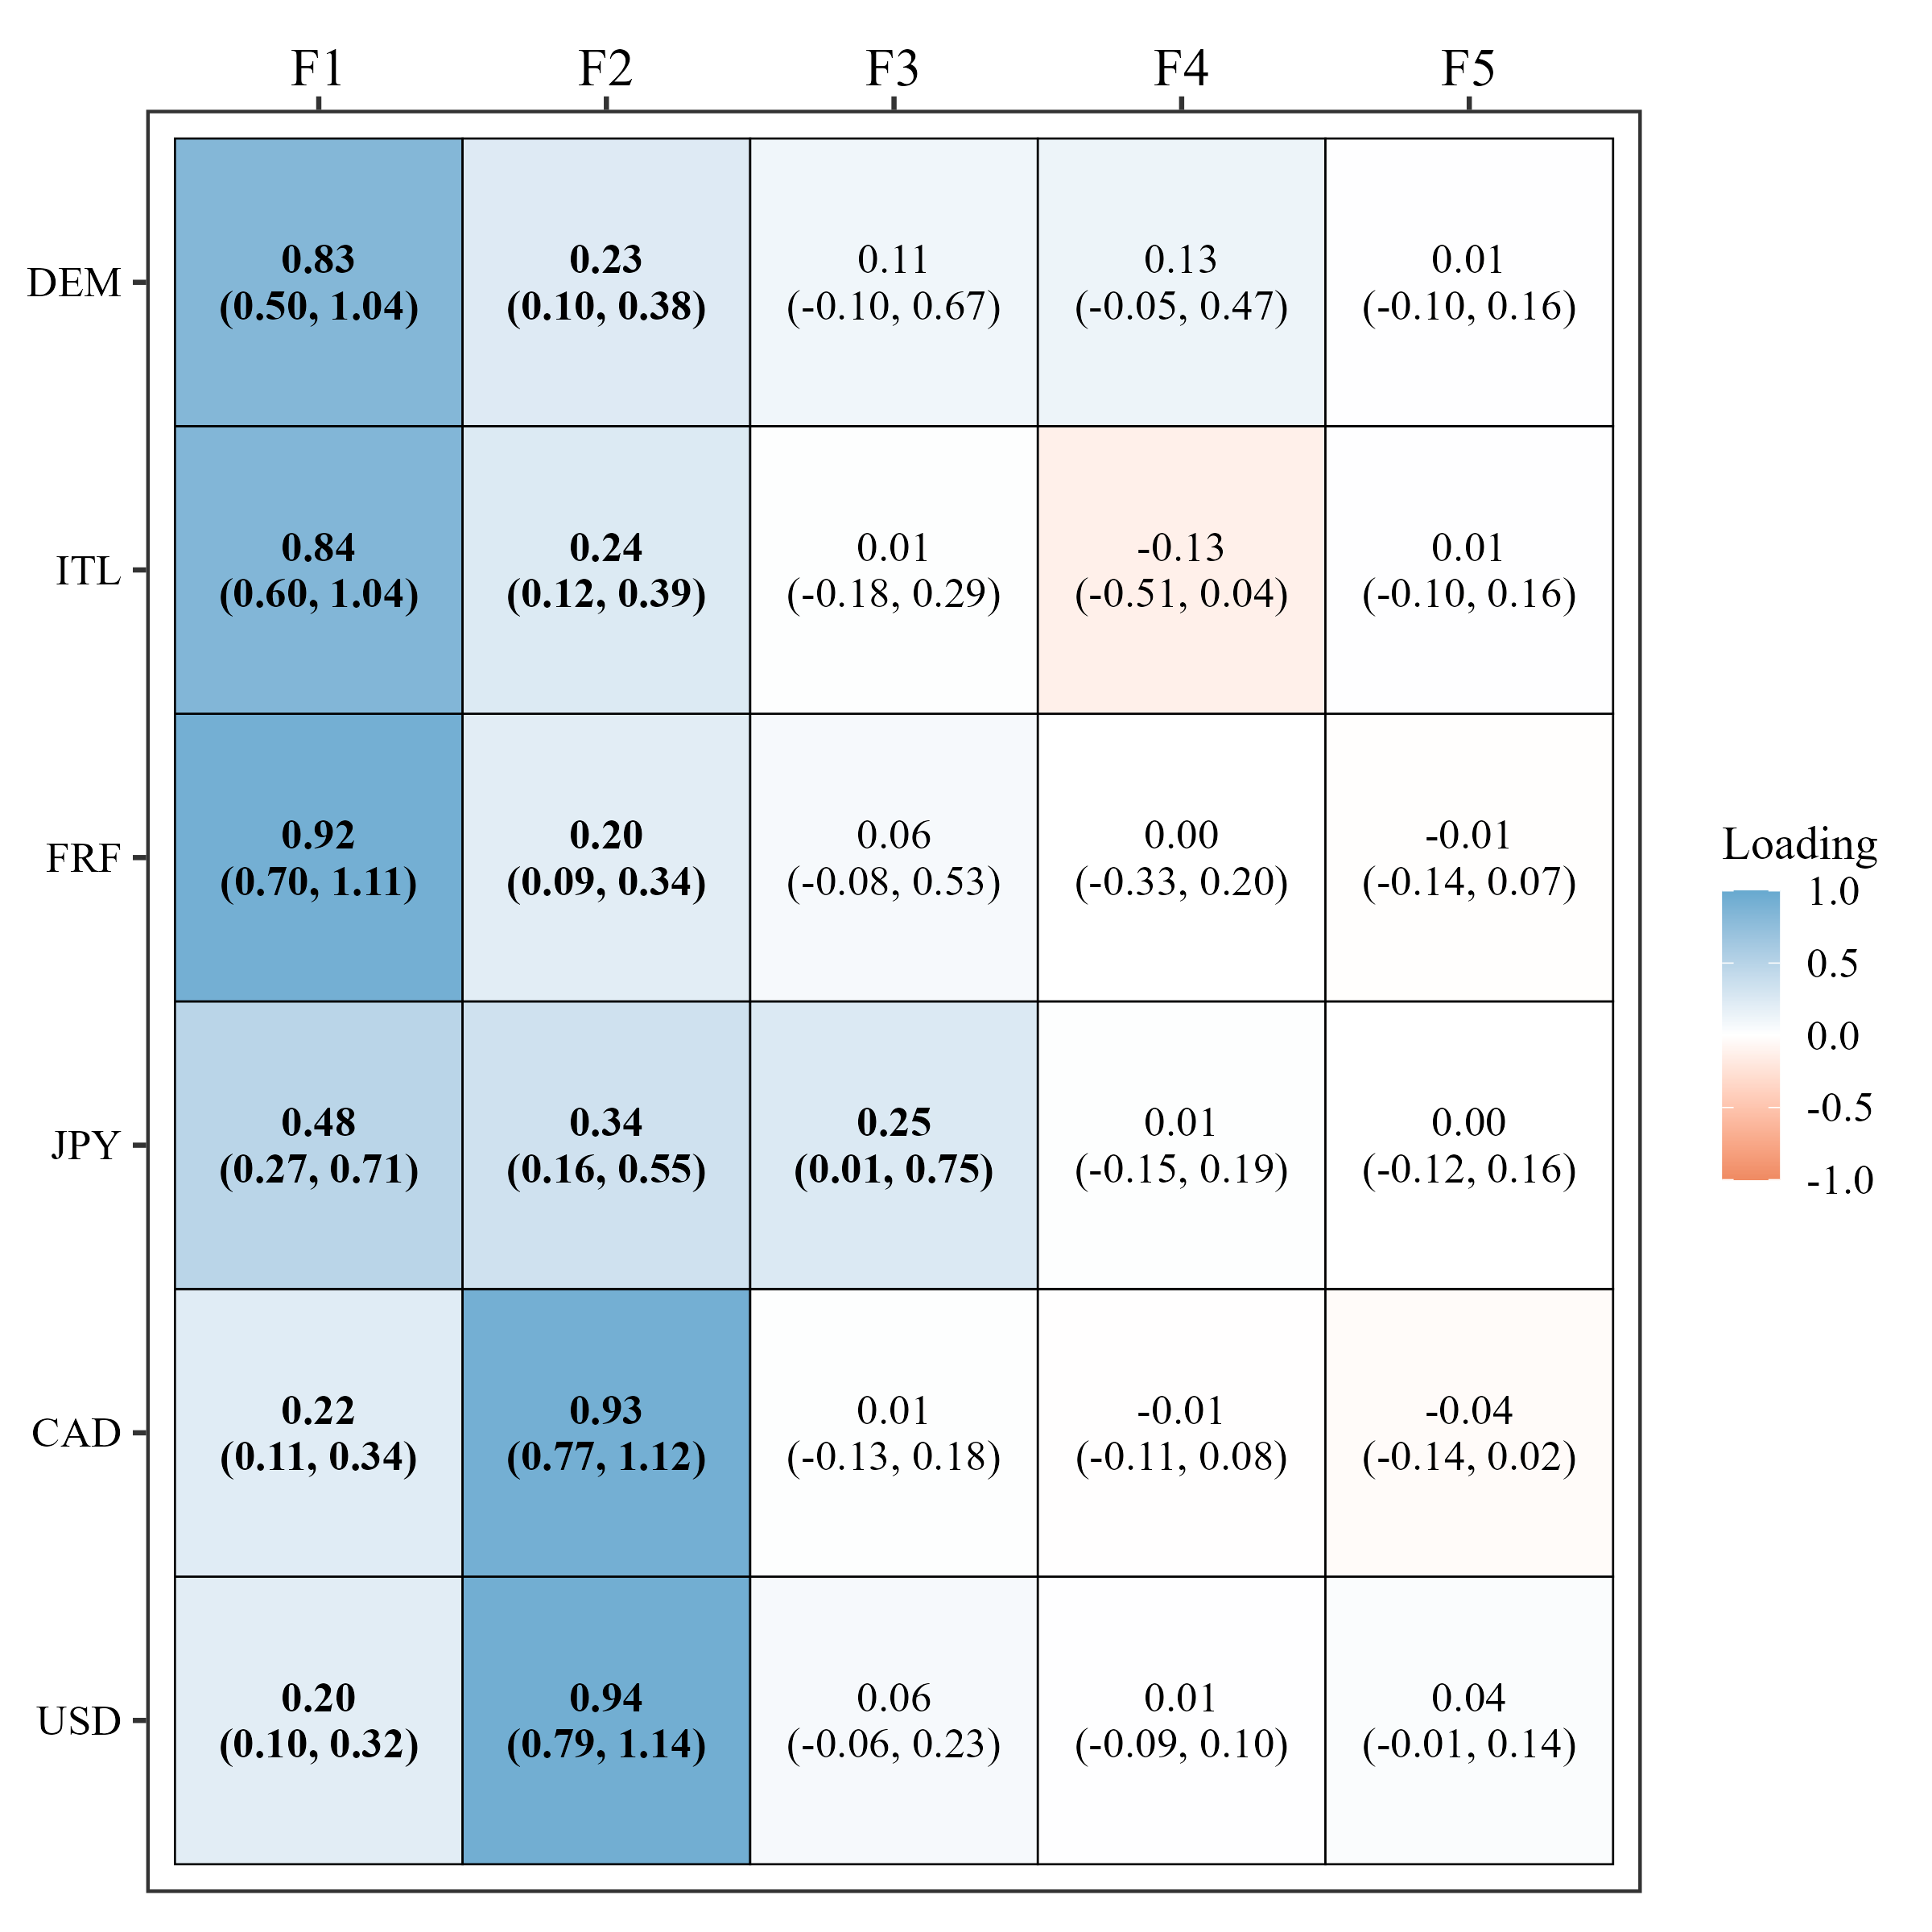
\includegraphics[width=6in,height=6in]{../Figures/factor_loading_matrix.png}

\end{figure}%

\section{Discussion}\label{discussion}

The primary contribution of this work is an exact and scalable solution
to rotational indeterminacy in Bayesian EFA. Until now, the state of the
art faced a clear limitation: exact post-processing methods were
computationally demanding even in low-dimensional settings and quickly
became prohibitive as dimensionality increased, leaving approximate
methods as the only available option. By reducing sign-permutation
alignment to a single LAP, the algorithm introduced here (Algorithm
\ref{alg:efficient-rsp}) makes exact optimization feasible precisely in
the high-dimensional settings where exact solutions have so far been out
of reach.

This efficiency also supports extensions to complex latent structures.
Papastamoulis and Ntzoufras
(\citeproc{ref-papastamoulis2022identifiability}{2022}) discusses
alignment in mixtures of factor analyzers, while Poworoznek et al.
(\citeproc{ref-Poworoznek2025}{2025}) outline strategies for dynamic
factor models and multiview settings. At the same time, E-RSP brings
clear benefits even in the simplest unrestricted factor model. By
treating identification as post-processing, the method yields a Bayesian
EFA workflow that directly parallels frequentist EFA practice in
empirical settings: fit the unrestricted model first, then rotate for
interpretation. We expect this close parallel to facilitate the
transition for researchers familiar with frequentist EFA to Bayesian
EFA, where proper prior specification can help address well-known
frequentist issues such as Heywood cases
(\citeproc{ref-heywood1931finite}{Heywood, 1931}) and non-positive
definite covariance estimates
(\citeproc{ref-Lorenzo-Seva2021}{Lorenzo-Seva \& Ferrando, 2021}).

However, we consider that the most immediate impact lies in factor
models where Bayesian estimation is not merely convenient but often
necessary, as in cognitive psychometrics
(\citeproc{ref-Batchelder1998}{Batchelder, 1998};
\citeproc{ref-Vandekerckhove2014}{Vandekerckhove, 2014}). In this area,
Hierarchical Factor Models are increasingly used to link latent factors
with hierarchical linear models (\citeproc{ref-rey-saez2025}{Rey-Sáez et
al., 2025}; \citeproc{ref-Rouder2025HFM}{Rouder et al., 2025};
\citeproc{ref-rouder2025randomeffects}{Rouder, 2025}) or hierarchical
cognitive process models like the Drift Diffusion Model
(\citeproc{ref-Stevenson2024}{Stevenson et al., 2024},
\citeproc{ref-Stevenson2025group}{2025};
\citeproc{ref-Vandekerckhove2014}{Vandekerckhove, 2014}). The practical
demand for exact yet fast alignment is already reflected in applied
software: for example, the \texttt{EMC2} package
(\citeproc{ref-EMC2}{Stevenson et al., 2026}) implements a parallelized
version of exact RSP to enable rapid post-processing without giving up
exactness. Our method addresses the same need while removing the
combinatorial bottleneck that makes exhaustive RSP costly as \(M\)
grows.

Alongside these practical gains, it is important to note a general
consideration in Bayesian factor models, regardless of the specific
identification strategy. In practice, we place prior distributions on
unrotated, non-identified \(\mathbf\Lambda\), whereas interpretation
relies on a rotated and identified solution. Since obtaining an
identified \(\mathbf\Lambda\) requires additional post-sampling steps,
the specified prior on the non-identified \(\mathbf\Lambda\) does not
translate transparently into the implied prior on the identified
\(\mathbf\Lambda\) we ultimately report. This issue is what Merkle et
al. (\citeproc{ref-Merkle2023}{2023}) term \emph{opaque prior
distributions}, and it can arise even in more restrictive factor models,
such as Bayesian confirmatory factor analysis, where sign indeterminacy
is the sole remaining source of non-identifiability. Post-processing
algorithms that begin with an initial Varimax rotation are also affected
by this issue, since priors are generally not invariant under this
transformation (\citeproc{ref-Poworoznek2025}{Poworoznek et al., 2025}).
The main practical consequence is that procedures relying on the prior
specification can yield misleading results. For instance, prior
predictive checks, simulation-based calibration, and Bayes factors
targeting specific loading hypotheses may inadvertently evaluate the
wrong implied prior once identification and relabeling steps are
applied.

Finally, to facilitate widespread adoption of E-RSP in applied research,
we provide an optimized C++ implementation that is publicly available
through the open-source R package \texttt{BayesEFA}. Because it requires
only posterior draws of the loading matrix as input, E-RSP can be
integrated straightforwardly into existing Bayesian factor model
workflows. This enables researchers to address rotational indeterminacy
with an exact post-processing approach in settings where exact solutions
have not previously been feasible.

\newpage

\section{References}\label{references}

\phantomsection\label{refs}
\begin{CSLReferences}{1}{0}
\bibitem[\citeproctext]{ref-aguilar2000bayesian}
Aguilar, O., \& West, M. (2000). Bayesian dynamic factor models and
portfolio allocation. \emph{Journal of Business \& Economic Statistics},
\emph{18}(3), 338--357. \url{http://www.jstor.org/stable/1392266}

\bibitem[\citeproctext]{ref-anderson1956statistical}
Anderson, T. W., \& Rubin, H. (1956). Statistical inference in factor
analysis. \emph{Proceedings of the Third Berkeley Symposium on
Mathematical Statistics and Probability}, \emph{5}, 111--150.

\bibitem[\citeproctext]{ref-Asman2016}
Aßmann, C., Boysen-Hogrefe, J., \& Pape, M. (2016). Bayesian analysis of
static and dynamic factor models: An ex-post approach towards the
rotation problem. \emph{Journal of Econometrics}, \emph{192}(1),
190--206.
https://doi.org/\url{https://doi.org/10.1016/j.jeconom.2015.10.010}

\bibitem[\citeproctext]{ref-Batchelder1998}
Batchelder, W. H. (1998). Multinomial processing tree models and
psychological assessment {[}Article{]}. \emph{Psychological Assessment},
\emph{10}(4), 331--344. \url{https://doi.org/10.1037/1040-3590.10.4.331}

\bibitem[\citeproctext]{ref-bhattacharya2011sparse}
Bhattacharya, A., \& Dunson, D. B. (2011). Sparse {Bayesian} infinite
factor models. \emph{Biometrika}, \emph{98}(2), 291--306.
\url{https://doi.org/10.1093/biomet/asr013}

\bibitem[\citeproctext]{ref-vanBork2024}
Bork, R. van, Rhemtulla, M., Sijtsma, K., \& Borsboom, D. (2024). A
causal theory of error scores. \emph{Psychological Methods},
\emph{29}(4), 807--826. \url{https://doi.org/10.1037/met0000521}

\bibitem[\citeproctext]{ref-Carvalho2008}
Carvalho, C. M., Chang, J., Lucas, J. E., Nevins, J. R., Wang, Q., \&
West, M. (2008). High-dimensional sparse factor modeling: Applications
in gene expression genomics. \emph{Journal of the American Statistical
Association}, \emph{103}(484), 1438--1456.
\url{https://doi.org/10.1198/016214508000000869}

\bibitem[\citeproctext]{ref-SimDesign}
Chalmers, R. P., \& Adkins, M. C. (2020). Writing effective and reliable
{Monte Carlo} simulations with the {SimDesign} package. \emph{The
Quantitative Methods for Psychology}, \emph{16}(4), 248--280.
\url{https://doi.org/10.20982/tqmp.16.4.p248}

\bibitem[\citeproctext]{ref-Chen2021}
Chen, J. (2021). A bayesian regularized approach to exploratory factor
analysis in one step. \emph{Structural Equation Modeling: A
Multidisciplinary Journal}, \emph{28}(4), 518--528.
\url{https://doi.org/10.1080/10705511.2020.1854763}

\bibitem[\citeproctext]{ref-conti2014bayesian}
Conti, G., Frühwirth-Schnatter, S., Heckman, J. J., \& Piatek, R.
(2014). {Bayesian} exploratory factor analysis. \emph{Journal of
Econometrics}, \emph{183}(1), 31--57.
\url{https://doi.org/10.1016/j.jeconom.2014.06.008}

\bibitem[\citeproctext]{ref-erosheva2017dealing}
Erosheva, E. A., \& Curtis, S. M. (2017). Dealing with reflection
invariance in bayesian factor analysis. \emph{Psychometrika},
\emph{82}(2), 295--307. \url{https://doi.org/10.1007/s11336-017-9564-y}

\bibitem[\citeproctext]{ref-Fan2008}
Fan, J., Fan, Y., \& Lv, J. (2008). High dimensional covariance matrix
estimation using a factor model. \emph{Journal of Econometrics},
\emph{147}(1), 186--197.
https://doi.org/\url{https://doi.org/10.1016/j.jeconom.2008.09.017}

\bibitem[\citeproctext]{ref-mvnfast}
Fasiolo, M. (2014). \emph{An introduction to mvnfast. R package version
0.2.8.} University of Bristol.
\url{https://CRAN.R-project.org/package=mvnfast}

\bibitem[\citeproctext]{ref-fokoue2003mixtures}
Fokoué, E., \& Titterington, D. (2003). Mixtures of factor analysers.
Bayesian estimation and inference by stochastic simulation.
\emph{Machine Learning}, \emph{50}(1), 73--94.
\url{https://doi.org/10.1023/A:1020297828025}

\bibitem[\citeproctext]{ref-Fontanella2019}
Fontanella, L., Fontanella, S., Valentini, P., \& Trendafilov, N.
(2019). Simple structure detection through bayesian exploratory
multidimensional IRT models. \emph{Multivariate Behavioral Research},
\emph{54}(1), 100--112.
\url{https://doi.org/10.1080/00273171.2018.1496317}

\bibitem[\citeproctext]{ref-econometrics11040026}
Frühwirth-Schnatter, S., Hosszejni, D., \& Lopes, H. F. (2023). When it
counts--econometric identification of the basic factor model based on
GLT structures. \emph{Econometrics}, \emph{11}(4).
\url{https://doi.org/10.3390/econometrics11040026}

\bibitem[\citeproctext]{ref-Fruxfchwirth-Schnatter2025}
Frühwirth-Schnatter, S., Hosszejni, D., \& Lopes, H. F. (2025). {Sparse
Bayesian Factor Analysis When the Number of Factors Is Unknown (with
Discussion)}. \emph{Bayesian Analysis}, \emph{20}(1), 213--344.
\url{https://doi.org/10.1214/24-BA1423}

\bibitem[\citeproctext]{ref-geweke1996measuring}
Geweke, J., \& Zhou, G. (1996). Measuring the pricing error of the
arbitrage pricing theory. \emph{The Review of Financial Studies},
\emph{9}(2), 557--587. \url{http://www.jstor.org/stable/2962214}

\bibitem[\citeproctext]{ref-Gronau2020}
Gronau, Q. F., Singmann, H., \& Wagenmakers, E.-J. (2020).
Bridgesampling: An r package for estimating normalizing constants.
\emph{Journal of Statistical Software}, \emph{92}(10), 1â€``29.
\url{https://doi.org/10.18637/jss.v092.i10}

\bibitem[\citeproctext]{ref-heywood1931finite}
Heywood, H. B. (1931). On finite sequences of real numbers.
\emph{Proceedings of the Royal Society of London. Series A, Containing
Papers of a Mathematical and Physical Character}, \emph{134}, 486--501.
\url{https://doi.org/10.1098/rspa.1931.0209}

\bibitem[\citeproctext]{ref-JennrichSampson1966}
Jennrich, R. I., \& Sampson, P. F. (1966). Rotation for simple loadings.
\emph{Psychometrika}, \emph{31}(3), 313--323.
\url{https://doi.org/10.1007/BF02289465}

\bibitem[\citeproctext]{ref-joreskog1969general}
Jöreskog, K. G. (1969). A general approach to confirmatory maximum
likelihood factor analysis. \emph{Psychometrika}, \emph{34}(2),
183--202.

\bibitem[\citeproctext]{ref-kaiser1958varimax}
Kaiser, H. F. (1958). The varimax criterion for analytic rotation in
factor analysis. \emph{Psychometrika}, \emph{23}(3), 187--200.
\url{https://doi.org/10.1007/BF02289233}

\bibitem[\citeproctext]{ref-Kaufmann2017}
Kaufmann, S., \& Schumacher, C. (2017). Identifying relevant and
irrelevant variables in sparse factor models. \emph{Journal of Applied
Econometrics}, \emph{32}(6), 1123--1144.
https://doi.org/\url{https://doi.org/10.1002/jae.2566}

\bibitem[\citeproctext]{ref-Knowles2011}
Knowles, D., \& Ghahramani, Z. (2011). {Nonparametric Bayesian sparse
factor models with application to gene expression modeling}. \emph{The
Annals of Applied Statistics}, \emph{5}(2B), 1534--1552.
\url{https://doi.org/10.1214/10-AOAS435}

\bibitem[\citeproctext]{ref-Kuhn1955Hungarian}
Kuhn, H. W. (1955). The {Hungarian} method for the assignment problem.
\emph{Naval Research Logistics Quarterly}, \emph{2}(1--2), 83--97.
\url{https://doi.org/10.1002/nav.3800020109}

\bibitem[\citeproctext]{ref-Legramanti2020}
Legramanti, S., Durante, D., \& Dunson, D. B. (2020). Bayesian
cumulative shrinkage for infinite factorizations. \emph{Biometrika},
\emph{107}(3), 745--752. \url{https://doi.org/10.1093/biomet/asaa008}

\bibitem[\citeproctext]{ref-Little1963}
Little, J. D. C., Murty, K. G., Sweeney, D. W., \& Karel, C. (1963). An
algorithm for the traveling salesman problem. \emph{Operations
Research}, \emph{11}(6), 972--989.
\url{http://www.jstor.org/stable/167836}

\bibitem[\citeproctext]{ref-lopes2004bayesian}
Lopes, H. F., \& West, M. (2004). Bayesian model assessment in factor
analysis. \emph{Statistica Sinica}, \emph{14}(1), 41--67.
\url{http://www.jstor.org/stable/24307179}

\bibitem[\citeproctext]{ref-Lorenzo-Seva2021}
Lorenzo-Seva, U., \& Ferrando, P. J. (2021). Not positive definite
correlation matrices in exploratory item factor analysis: Causes,
consequences and a proposed solution. \emph{Structural Equation
Modeling: A Multidisciplinary Journal}, \emph{28}(1), 138--147.
\url{https://doi.org/10.1080/10705511.2020.1735393}

\bibitem[\citeproctext]{ref-lucas2006sparse}
Lucas, J., Carvalho, C., Wang, Q., Bild, A., Nevins, J. R., \& West, M.
(2006). Sparse statistical modelling in gene expression genomics. In
K.-A. Do, P. Müller, \& M. Vannucci (Eds.), \emph{Bayesian inference for
gene expression and proteomics} (pp. 155--176). Cambridge University
Press.

\bibitem[\citeproctext]{ref-Marin2005}
Marin, J.-M., Mengersen, K., \& Robert, C. P. (2005). Bayesian modelling
and inference on mixtures of distributions. In D. K. Dey \& C. R. Rao
(Eds.), \emph{Bayesian thinking} (Vol. 25, pp. 459--507). Elsevier.
https://doi.org/\url{https://doi.org/10.1016/S0169-7161(05)25016-2}

\bibitem[\citeproctext]{ref-Mavridis2014}
Mavridis, D., \& Ntzoufras, I. (2014). Stochastic search item selection
for factor analytic models. \emph{British Journal of Mathematical and
Statistical Psychology}, \emph{67}(2), 284--303.
https://doi.org/\url{https://doi.org/10.1111/bmsp.12019}

\bibitem[\citeproctext]{ref-Meng1996}
Meng, X.-L., \& Wong, W. H. (1996). SIMULATING RATIOS OF NORMALIZING
CONSTANTS VIA a SIMPLE IDENTITY: A THEORETICAL EXPLORATION.
\emph{Statistica Sinica}, \emph{6}(4), 831--860.
\url{http://www.jstor.org/stable/24306045}

\bibitem[\citeproctext]{ref-Merkle2023}
Merkle, E. C., Ariyo, O., Winter, S. D., \& Garnier-Villarreal, M.
(2023). Opaque prior distributions in bayesian latent variable models.
\emph{Methodology}, \emph{19}(3).
\url{https://doi.org/10.5964/meth.11167}

\bibitem[\citeproctext]{ref-millsap2001statistical}
Millsap, R. E. (2001). When trivial constraints are not trivial: The
choice of uniqueness constraints in confirmatory factor analysis.
\emph{Structural Equation Modeling: A Multidisciplinary Journal},
\emph{8}(1), 1--17. \url{https://doi.org/10.1207/S15328007SEM0801_1}

\bibitem[\citeproctext]{ref-nirwan19a}
Nirwan, R., \& Bertschinger, N. (2019). Rotation invariant householder
parameterization for {B}ayesian {PCA}. In K. Chaudhuri \& R.
Salakhutdinov (Eds.), \emph{Proceedings of the 36th international
conference on machine learning} (Vol. 97, pp. 4820--4828). PMLR.
\url{https://proceedings.mlr.press/v97/nirwan19a.html}

\bibitem[\citeproctext]{ref-papastamoulis2022identifiability}
Papastamoulis, P., \& Ntzoufras, I. (2022). On the identifiability of
bayesian factor analytic models. \emph{Statistics and Computing},
\emph{32}(2), 23. \url{https://doi.org/10.1007/s11222-022-10084-4}

\bibitem[\citeproctext]{ref-infinitefactor}
Poworoznek, E. (2020). \emph{Infinitefactor: Bayesian infinite factor
models}. \url{https://CRAN.R-project.org/package=infinitefactor}

\bibitem[\citeproctext]{ref-Poworoznek2025}
Poworoznek, E., Anceschi, N., Ferrari, F., \& Dunson, D. (2025).
{Efficiently Resolving Rotational Ambiguity in Bayesian Matrix Sampling
with Matching}. \emph{Bayesian Analysis}, 1--22.
\url{https://doi.org/10.1214/25-BA1544}

\bibitem[\citeproctext]{ref-Quintero2024}
Quintero, A., Lesaffre, E., \& Verbeke, G. (2024). Bayesian exploratory
factor analysis via gibbs sampling. \emph{Journal of Educational and
Behavioral Statistics}, \emph{49}(1), 121--142.
\url{https://doi.org/10.3102/10769986231176023}

\bibitem[\citeproctext]{ref-Rcite}
R Core Team. (2025). \emph{R: A language and environment for statistical
computing}. R Foundation for Statistical Computing.
\url{https://www.R-project.org/}

\bibitem[\citeproctext]{ref-revuelta2022bayesian}
Revuelta, J., Hidalgo, B., \& Alcazar-Córcoles, M. Á. (2022). Bayesian
estimation and testing of a beta factor model for bounded continuous
variables. \emph{Multivariate Behavioral Research}, \emph{57}(1),
57--78. \url{https://doi.org/10.1080/00273171.2020.1805582}

\bibitem[\citeproctext]{ref-Revuelta2017}
Revuelta, J., \& Ximénez, C. (2017). Bayesian dimensionality assessment
for the multidimensional nominal response model. \emph{Frontiers in
Psychology}, \emph{Volume 8 - 2017}.
\url{https://doi.org/10.3389/fpsyg.2017.00961}

\bibitem[\citeproctext]{ref-BayesEFA}
Rey-Sáez, R. (2026). \emph{BayesEFA: Bayesian exploratory factor
analysis using 'stan'}. \url{https://ricardoreysaez.github.io/BayesEFA/}

\bibitem[\citeproctext]{ref-rey-saez2025}
Rey-Sáez, R., Franco-Martínez, A., Revuelta, J., \& Vadillo, M. A.
(2025). A unified framework for psychometrics in experimental
psychology: The standardized generalized hierarchical factor model.
\emph{PsyArXiv}. \url{https://doi.org/10.31234/osf.io/gv6k7_v1}

\bibitem[\citeproctext]{ref-rockova2016fast}
Ročková, V., \& George, E. I. (2016). Fast {Bayesian} factor analysis
via automatic rotations to sparsity. \emph{Journal of the American
Statistical Association}, \emph{111}(516), 1608--1622.
\url{https://doi.org/10.1080/01621459.2015.1100620}

\bibitem[\citeproctext]{ref-rouder2025randomeffects}
Rouder, J. N. (2025). \emph{Random-effects psychophysics for studying
individual differences in perception}. \url{https://osf.io/7zb6p_v1}.

\bibitem[\citeproctext]{ref-Rouder2025HFM}
Rouder, J. N., Mehrvarz, M., \& Stevenson, N. (2025). Hierarchical
factor models for analysis in experimental designs. \emph{PsyArXiv}.
\url{https://doi.org/10.31234/osf.io/cetwz_v3}

\bibitem[\citeproctext]{ref-Schonemann1966Procrustes}
Schönemann, P. H. (1966). A generalized solution of the orthogonal
{P}rocrustes problem. \emph{Psychometrika}, \emph{31}(1), 1--10.
\url{https://doi.org/10.1007/BF02289451}

\bibitem[\citeproctext]{ref-EMC2}
Stevenson, N., Donzallaz, M., Heathcote, A., \& Miletić, S. (2026).
\emph{EMC2: Bayesian hierarchical analysis of cognitive models of
choice}. \url{https://doi.org/10.32614/CRAN.package.EMC2}

\bibitem[\citeproctext]{ref-Stevenson2024}
Stevenson, N., Heathcote, A., Forstmann, B., \& Matzke, D. (2024).
Efficient bayesian hierarchical factor analysis for model-based
psychological research. \emph{PsyArXiv}.
\url{https://doi.org/10.31234/osf.io/zangj}

\bibitem[\citeproctext]{ref-Stevenson2025group}
Stevenson, N., Innes, R. J., Gronau, Q. F., Miletić, S., Heathcote, A.,
Forstmann, B. U., \& Brown, S. D. (2025). Using group level factor
models to resolve high dimensionality in model-based sampling.
\emph{Psychological Methods}, \emph{30}(6), 1218--1241.
\url{https://doi.org/10.1037/met0000618}

\bibitem[\citeproctext]{ref-thurstone1947multiple}
Thurstone, L. L. (1947). \emph{Multiple-factor analysis: A development
and expansion of the vectors of mind}. University of Chicago Press.

\bibitem[\citeproctext]{ref-Vandekerckhove2014}
Vandekerckhove, J. (2014). A cognitive latent variable model for the
simultaneous analysis of behavioral and personality data. \emph{Journal
of Mathematical Psychology}, \emph{60}, 58--71.
\url{https://doi.org/10.1016/j.jmp.2014.06.004}

\end{CSLReferences}






\end{document}
